%%%%%%%%%%%%%%%%%%%%
%%% Document
%%%%%%%%%%%%%%%%%%%%
\documentclass[pdftex, a4paper,11pt, twoside, ngerman]{report}
% \documentclass[11pt,xcolor=dvipsnames]{beamer}

% für deutsche zeichen äüö ohne kile auto-ersetzen
% \usepackage[utf8x]{inputenc}

% kile auto-ersetzen: einstellungen->latex:general-> hacken bei special
% characters
% \usepackage[ansinew]{inputenc}
% \usepackage[UKenglish]{babel}          %Englisch
\usepackage[ngerman]{babel}          %Deutsch


%%%%%%%%%%
%%% Geometry
%%%%%%%%%%
% \usepackage{showframe}
\usepackage[scale=0.8, hmarginratio=4:2]{geometry}
  \geometry{textheight=1.05\textheight, textwidth=.95\textwidth,
            marginparwidth=25 pt}



%%%%%%%%%%
%%% Packages (aus header datei)
%%%%%%%%%%
\IfFileExists{header_TobiasBrauell-DOCUMENT.tex}{
    % Copyright © 2014 Tobias Brauell <tobiasbrauell@gmail.com>

% This is my general purpose LaTeX header file for writing German documents.
% Ideally, you include this using a simple ``\input{header.tex}`` in your main
% document and start with ``\title`` and ``\begin{document}`` afterwards.

% If you need to add additional packages, I recommend not doing this in this
% file, but in your main document. That way, you can just drop in a new
% ``header.tex`` and get all the new commands without having to merge manually.

%%%%%%%%%%%%%%%%%%%%%%%%%%%%%
%%% Locale, date
%%%%%%%%%%%%%%%%%%%%%%%%%%%%%
\usepackage[UKenglish]{isodate}



%%%%%%%%%%%%%%%%%%%%%%%%%%%%%
%%% Margins and other spacing
%%%%%%%%%%%%%%%%%%%%%%%%%%%%%
\usepackage[activate]{pdfcprot}
% \usepackage[parfill]{parskip}
\usepackage{setspace}
  \setlength{\columnsep}{2 cm}
  \setlength{\parindent}{0 pt}


%%%%%%%%%%%%%%%%%%%%%%%%%%%%%
%%% Input encoding
%%%%%%%%%%%%%%%%%%%%%%%%%%%%%
\usepackage[T1]{fontenc}
\usepackage[utf8x]{inputenc}



%%%%%%%%%%%%%%%%%%%%%%%%%%%%%
%%% Indexing
%%%%%%%%%%%%%%%%%%%%%%%%%%%%%
\usepackage{makeidx}
  \makeindex



%%%%%%%%%%%%%%%%%%%%%%%%%%%%%
%%% Blindtext
%%%%%%%%%%%%%%%%%%%%%%%%%%%%%
\usepackage{blindtext}


%%%%%%%%%%%%%%%%%%%%%%%%%%%%%
%%% Global Counter
%%%%%%%%%%%%%%%%%%%%%%%%%%%%%



%%%%%%%%%%%%%%%%%%%%%%%%%%%%%
%%% Geometry
%%%%%%%%%%%%%%%%%%%%%%%%%%%%%
\usepackage{layout}
% \usepackage[scale=0.8]{geometry}
%   \geometry{textheight=1.05\textheight, marginparwidth=50 pt}

% \usepackage{multirow}
% \usepackage{dcolumn}



%%%%%%%%%%%%%%%%%%%%%%%%%%%%%
%%% Pagestyle
%%%%%%%%%%%%%%%%%%%%%%%%%%%%%
% \usepackage{fancyhdr}
% \usepackage{microtype} 

% \pagestyle{fancy}



%%%%%%%%%%%%%%%%%%%%%%%%%%%%%
%%% Fonts/Colors
%%%%%%%%%%%%%%%%%%%%%%%%%%%%%
\usepackage{lmodern}
\usepackage{xcolor}
% This replaces all fonts with Bitstream Charter, Bitstream Vera Sans and
% Bitstream Vera Mono. Math will be rendered in Charter.
% \usepackage[charter, greekuppercase=italicized]{mathdesign}
% \usepackage{beramono}
% \usepackage{berasans}

% Bold, sans-serif tensors. This fragment is taken from “egreg” from
% http://tex.stackexchange.com/a/82747/8945 and licensed under `CC-BY-SA
% <https://creativecommons.org/licenses/by-sa/3.0/>`_.
% \usepackage{bm}
%   \DeclareMathAlphabet{\mathsfit}{\encodingdefault}{\sfdefault}{m}{sl}
%   \SetMathAlphabet{\mathsfit}{bold}{\encodingdefault}{\sfdefault}{bx}{sl}
%   \newcommand{\tens}[1]{\bm{\mathsfit{#1}}}

% Bold vectors.
% \renewcommand{\vec}[1]{\boldsymbol{#1}}



%%%%%%%%%%%%%%%%%%%%%%%%%%%%%
%%% Code/Listings
%%%%%%%%%%%%%%%%%%%%%%%%%%%%%
\usepackage{listings}



%%%%%%%%%%%%%%%%%%%%%%%%%%%%%
%%% Enumerations
%%%%%%%%%%%%%%%%%%%%%%%%%%%%%
\usepackage{enumitem}
% \usepackage{paralist}


%%%%%%%%%%%%%%%%%%%%%%%%%%%%%
%%% Figures
%%%%%%%%%%%%%%%%%%%%%%%%%%%%%
% \usepackage[pdftex]{graphicx}
\usepackage{graphicx}
\usepackage{epsfig}
\usepackage{epstopdf}
\usepackage{subfigure}
\usepackage{wrapfig}
\makeatletter \newcommand\hyper@makecurrent[1]{} \makeatother
\usepackage{caption}
% \usepackage{subcaption}

\addto\captionsUKenglish{\renewcommand{\figurename}{Fig.}}
\addto\captionsngerman{\renewcommand{\figurename}{Abb.}}



%%%%%%%%%%%%%%%%%%%%%%%%%%%%%
%%% PDF Pages
%%%%%%%%%%%%%%%%%%%%%%%%%%%%%
\usepackage{pdfpages}



%%%%%%%%%%%%%%%%%%%%%%%%%%%%%
%%% Personal Graphics
%%%%%%%%%%%%%%%%%%%%%%%%%%%%%
\usepackage{tikz}
% \usepackage{tikz-3dplot}
  \usetikzlibrary{calc}
  \usetikzlibrary{decorations.markings}



%%%%%%%%%%%%%%%%%%%%%%%%%%%%%
%%% Math
%%%%%%%%%%%%%%%%%%%%%%%%%%%%%
\usepackage{amsmath}
\usepackage{amssymb}
\usepackage{mathtools}
\usepackage{dcolumn}
\usepackage{siunitx}
% \usepackage{feynmf}



%%%%%%%%%%%%%%%%%%%%%%%%%%%%%
%%% Referenzen
%%%%%%%%%%%%%%%%%%%%%%%%%%%%%
\usepackage{hyperref}
\usepackage{url}
% \usepackage{cleveref}%\label{abc}--\cref{abc} \Cref{abc[,def]}-und \crefrange{abc}{def}-bis
\usepackage[english]{cleveref}%\label{abc}--\cref{abc} \Cref{abc[,def]}-und \crefrange{abc}{def}-bis



%%%%%%%%%%%%%%%%%%%%%%%%%%%%%
%%% Table's
%%%%%%%%%%%%%%%%%%%%%%%%%%%%%
\usepackage{rotating}
\usepackage{longtable}
\usepackage{multirow}
\usepackage{tabularx}
  \newcolumntype{L}[1]{>{\raggedright\arraybackslash}p{#1}} % linksbündig mit Breitenangabe
  \newcolumntype{C}[1]{>{\centering\arraybackslash}p{#1}} % zentriert mit Breitenangabe
  \newcolumntype{R}[1]{>{\raggedleft\arraybackslash}p{#1}} % rechtsbündig mit Breitenangabe



%%%%%%%%%%%%%%%%%%%%%%%%%%%%%
%%% Todo's
%%%%%%%%%%%%%%%%%%%%%%%%%%%%%
% \usepackage{xkeyval}
\usepackage{todonotes} %\todo{text} oder \todo[inline]{text}
%   \presetkeys{todonotes}{inline}{}
%   \let\todox\todo
%   \renewcommand\todo{1}{\todox[inline]{#1}}


%%%%%%%%%%%%%%%%%%%%%%%%%%%%%%%%%%%%%%%%%%%%%%%%%%%%%%%%%%
%%% Settings
%%%%%%%%%%%%%%%%%%%%%%%%%%%%%%%%%%%%%%%%%%%%%%%%%%%%%%%%%%
\usepackage{cancel}

\newcommand{\HRule}{\rule{\linewidth}{0.5mm}}



%%%%%%%%%%%%%%%%%%%%%%%%%%%%%
%%% Theme
%%%%%%%%%%%%%%%%%%%%%%%%%%%%%



%%%%%%%%%%%%%%%%%%%%%%%%%%%%%
%%% header
%%%%%%%%%%%%%%%%%%%%%%%%%%%%%
% \lhead{text}
% \chead{text}
% \rhead{text}



%%%%%%%%%%%%%%%%%%%%%%%%%%%%%
%%% footer
%%%%%%%%%%%%%%%%%%%%%%%%%%%%%
%%% Tobias Brauell       	Versuch....		Ruth Jacobs
% \renewcommand\footrulewidth{.4pt}
% \lfoot{\scriptsize Ruth Jacobs - Tobias Brauell \\ {\ \ \ \ \ \ \ \ \ \ } Gruppe $\alpha 9$} 
% \cfoot{\thepage\ / \ \pageref{LastPage}}
% \rfoot{\scriptsize Versuch 518: Höhenstrahlung \\ Tutor: Christoph Krieger {\ \ \ } } 



%%%%%%%%%%%%%%%%%%%%%%%%%%%%%
%%% Title Page
%%%%%%%%%%%%%%%%%%%%%%%%%%%%%
% \title[ITER { } International Thermonuclear Experimental Reactor]{\huge{\bf{ITER}} \\ \large{\bf{International Thermonuclear Experimental Reactor}}}
% \author[T. Brauell]{Tobias Brauell}
% \institute{Universität Bonn}
% 
% \date{09.~Dez.~2013}
% \logo{\includegraphics[width=.15\textwidth]{Figures/toplogo.png}}


}{
    % Copyright © 2014 Tobias Brauell <tobiasbrauell@gmail.com>

% This is my general purpose LaTeX header file for writing German documents.
% Ideally, you include this using a simple ``\input{header.tex}`` in your main
% document and start with ``\title`` and ``\begin{document}`` afterwards.

% If you need to add additional packages, I recommend not doing this in this
% file, but in your main document. That way, you can just drop in a new
% ``header.tex`` and get all the new commands without having to merge manually.

%%%%%%%%%%%%%%%%%%%%%%%%%%%%%
%%% Locale, date
%%%%%%%%%%%%%%%%%%%%%%%%%%%%%
\usepackage[UKenglish]{isodate}



%%%%%%%%%%%%%%%%%%%%%%%%%%%%%
%%% Margins and other spacing
%%%%%%%%%%%%%%%%%%%%%%%%%%%%%
\usepackage[activate]{pdfcprot}
% \usepackage[parfill]{parskip}
\usepackage{setspace}
  \setlength{\columnsep}{2 cm}
  \setlength{\parindent}{0 pt}


%%%%%%%%%%%%%%%%%%%%%%%%%%%%%
%%% Input encoding
%%%%%%%%%%%%%%%%%%%%%%%%%%%%%
\usepackage[T1]{fontenc}
\usepackage[utf8x]{inputenc}



%%%%%%%%%%%%%%%%%%%%%%%%%%%%%
%%% Indexing
%%%%%%%%%%%%%%%%%%%%%%%%%%%%%
\usepackage{makeidx}
  \makeindex



%%%%%%%%%%%%%%%%%%%%%%%%%%%%%
%%% Blindtext
%%%%%%%%%%%%%%%%%%%%%%%%%%%%%
\usepackage{blindtext}


%%%%%%%%%%%%%%%%%%%%%%%%%%%%%
%%% Global Counter
%%%%%%%%%%%%%%%%%%%%%%%%%%%%%



%%%%%%%%%%%%%%%%%%%%%%%%%%%%%
%%% Geometry
%%%%%%%%%%%%%%%%%%%%%%%%%%%%%
\usepackage{layout}
% \usepackage[scale=0.8]{geometry}
%   \geometry{textheight=1.05\textheight, marginparwidth=50 pt}

% \usepackage{multirow}
% \usepackage{dcolumn}



%%%%%%%%%%%%%%%%%%%%%%%%%%%%%
%%% Pagestyle
%%%%%%%%%%%%%%%%%%%%%%%%%%%%%
% \usepackage{fancyhdr}
% \usepackage{microtype} 

% \pagestyle{fancy}



%%%%%%%%%%%%%%%%%%%%%%%%%%%%%
%%% Fonts/Colors
%%%%%%%%%%%%%%%%%%%%%%%%%%%%%
\usepackage{lmodern}
\usepackage{xcolor}
% This replaces all fonts with Bitstream Charter, Bitstream Vera Sans and
% Bitstream Vera Mono. Math will be rendered in Charter.
% \usepackage[charter, greekuppercase=italicized]{mathdesign}
% \usepackage{beramono}
% \usepackage{berasans}

% Bold, sans-serif tensors. This fragment is taken from “egreg” from
% http://tex.stackexchange.com/a/82747/8945 and licensed under `CC-BY-SA
% <https://creativecommons.org/licenses/by-sa/3.0/>`_.
% \usepackage{bm}
%   \DeclareMathAlphabet{\mathsfit}{\encodingdefault}{\sfdefault}{m}{sl}
%   \SetMathAlphabet{\mathsfit}{bold}{\encodingdefault}{\sfdefault}{bx}{sl}
%   \newcommand{\tens}[1]{\bm{\mathsfit{#1}}}

% Bold vectors.
% \renewcommand{\vec}[1]{\boldsymbol{#1}}



%%%%%%%%%%%%%%%%%%%%%%%%%%%%%
%%% Code/Listings
%%%%%%%%%%%%%%%%%%%%%%%%%%%%%
\usepackage{listings}



%%%%%%%%%%%%%%%%%%%%%%%%%%%%%
%%% Enumerations
%%%%%%%%%%%%%%%%%%%%%%%%%%%%%
\usepackage{enumitem}
% \usepackage{paralist}


%%%%%%%%%%%%%%%%%%%%%%%%%%%%%
%%% Figures
%%%%%%%%%%%%%%%%%%%%%%%%%%%%%
% \usepackage[pdftex]{graphicx}
\usepackage{graphicx}
\usepackage{epsfig}
\usepackage{epstopdf}
\usepackage{subfigure}
\usepackage{wrapfig}
\makeatletter \newcommand\hyper@makecurrent[1]{} \makeatother
\usepackage{caption}
% \usepackage{subcaption}

\addto\captionsUKenglish{\renewcommand{\figurename}{Fig.}}
\addto\captionsngerman{\renewcommand{\figurename}{Abb.}}



%%%%%%%%%%%%%%%%%%%%%%%%%%%%%
%%% PDF Pages
%%%%%%%%%%%%%%%%%%%%%%%%%%%%%
\usepackage{pdfpages}



%%%%%%%%%%%%%%%%%%%%%%%%%%%%%
%%% Personal Graphics
%%%%%%%%%%%%%%%%%%%%%%%%%%%%%
\usepackage{tikz}
% \usepackage{tikz-3dplot}
  \usetikzlibrary{calc}
  \usetikzlibrary{decorations.markings}



%%%%%%%%%%%%%%%%%%%%%%%%%%%%%
%%% Math
%%%%%%%%%%%%%%%%%%%%%%%%%%%%%
\usepackage{amsmath}
\usepackage{amssymb}
\usepackage{mathtools}
\usepackage{dcolumn}
\usepackage{siunitx}
% \usepackage{feynmf}



%%%%%%%%%%%%%%%%%%%%%%%%%%%%%
%%% Referenzen
%%%%%%%%%%%%%%%%%%%%%%%%%%%%%
\usepackage{hyperref}
\usepackage{url}
% \usepackage{cleveref}%\label{abc}--\cref{abc} \Cref{abc[,def]}-und \crefrange{abc}{def}-bis
\usepackage[english]{cleveref}%\label{abc}--\cref{abc} \Cref{abc[,def]}-und \crefrange{abc}{def}-bis



%%%%%%%%%%%%%%%%%%%%%%%%%%%%%
%%% Table's
%%%%%%%%%%%%%%%%%%%%%%%%%%%%%
\usepackage{rotating}
\usepackage{longtable}
\usepackage{multirow}
\usepackage{tabularx}
  \newcolumntype{L}[1]{>{\raggedright\arraybackslash}p{#1}} % linksbündig mit Breitenangabe
  \newcolumntype{C}[1]{>{\centering\arraybackslash}p{#1}} % zentriert mit Breitenangabe
  \newcolumntype{R}[1]{>{\raggedleft\arraybackslash}p{#1}} % rechtsbündig mit Breitenangabe



%%%%%%%%%%%%%%%%%%%%%%%%%%%%%
%%% Todo's
%%%%%%%%%%%%%%%%%%%%%%%%%%%%%
% \usepackage{xkeyval}
\usepackage{todonotes} %\todo{text} oder \todo[inline]{text}
%   \presetkeys{todonotes}{inline}{}
%   \let\todox\todo
%   \renewcommand\todo{1}{\todox[inline]{#1}}


%%%%%%%%%%%%%%%%%%%%%%%%%%%%%%%%%%%%%%%%%%%%%%%%%%%%%%%%%%
%%% Settings
%%%%%%%%%%%%%%%%%%%%%%%%%%%%%%%%%%%%%%%%%%%%%%%%%%%%%%%%%%
\usepackage{cancel}

\newcommand{\HRule}{\rule{\linewidth}{0.5mm}}



%%%%%%%%%%%%%%%%%%%%%%%%%%%%%
%%% Theme
%%%%%%%%%%%%%%%%%%%%%%%%%%%%%



%%%%%%%%%%%%%%%%%%%%%%%%%%%%%
%%% header
%%%%%%%%%%%%%%%%%%%%%%%%%%%%%
% \lhead{text}
% \chead{text}
% \rhead{text}



%%%%%%%%%%%%%%%%%%%%%%%%%%%%%
%%% footer
%%%%%%%%%%%%%%%%%%%%%%%%%%%%%
%%% Tobias Brauell       	Versuch....		Ruth Jacobs
% \renewcommand\footrulewidth{.4pt}
% \lfoot{\scriptsize Ruth Jacobs - Tobias Brauell \\ {\ \ \ \ \ \ \ \ \ \ } Gruppe $\alpha 9$} 
% \cfoot{\thepage\ / \ \pageref{LastPage}}
% \rfoot{\scriptsize Versuch 518: Höhenstrahlung \\ Tutor: Christoph Krieger {\ \ \ } } 



%%%%%%%%%%%%%%%%%%%%%%%%%%%%%
%%% Title Page
%%%%%%%%%%%%%%%%%%%%%%%%%%%%%
% \title[ITER { } International Thermonuclear Experimental Reactor]{\huge{\bf{ITER}} \\ \large{\bf{International Thermonuclear Experimental Reactor}}}
% \author[T. Brauell]{Tobias Brauell}
% \institute{Universität Bonn}
% 
% \date{09.~Dez.~2013}
% \logo{\includegraphics[width=.15\textwidth]{Figures/toplogo.png}}


}



%%%%%%%%%%
%%%%%%%%%%
%%%%%%%%%%
\begin{document}
%   \layout
  
  
  
  %%%%%%%%%%%%%%%%%%%%
  %%%%%%%%%%%%%%%%%%%%
  %%%%%%%%%%%%%%%%%%%%
  %%%%%%%%%%%%%%%%%%%%%%%%%%%%%%%%%%%%%%%%%%%%%%%%%%%%%%%%%%
%%% Title Page - Bachelor Thesis
%%%%%%%%%%%%%%%%%%%%%%%%%%%%%%%%%%%%%%%%%%%%%%%%%%%%%%%%%%
\begin{titlepage}
  \thispagestyle{empty}
  \begin{center}

    % Upper part of the page. The '~' is needed because \\
    % only works if a paragraph has started.
%     \includegraphics[width=0.15\textwidth]{./logo}~\\[1cm]
    \begin{minipage}{0.5\textwidth}
      \begin{flushleft}
	
\includegraphics[width=.5\textwidth]{Figures/Logos/logoUNI.png}
      \end{flushleft}
    \end{minipage}%
    \begin{minipage}{0.5\textwidth}
      \begin{flushright}
	
\includegraphics[width=.5\textwidth]{Figures/Logos/logoPI.png}
      \end{flushright}
    \end{minipage}
    
    \vspace{25 pt}
    
    \textsc{\LARGE Rheinische Friedrich-Wilhelms-Universität Bonn}\\[1.5 cm]
    
    \vspace{50 pt}
    
    \textsc{\Large Praktikum 4 - Atome und Moleküle}\\[0.5 cm]

    % Title
    \HRule \\[0.4 cm]
    { \huge \bfseries Versuch 443 - Kernmagnetische Relaxation \\[0.4 cm] }

    \HRule \\[1.5 cm]

    % Author and supervisor
    \noindent
    \begin{minipage}{0.4\textwidth}
      \begin{flushleft} \large
	\emph{Authors:}\\
	Tobias \textsc{Brauell}\\
	Frederike \textsc{Schrödel}
      \end{flushleft}
    \end{minipage}%
    \begin{minipage}{0.4\textwidth}
      \begin{flushright} \large
	\emph{Supervisors:} \\
        Marcel \textsc{Bornstein} \\
        Scott \textsc{Reeve}
      \end{flushright}
    \end{minipage}

    \vfill

    % Bottom of the page
    \HRule \\[0.4 cm]
    {\large \today}

  \end{center}
\end{titlepage}
  %%%%%%%%%%%%%%%%%%%%
  
  
  
%   \setcounter{page}{2}
  
  \begin{chapter}*{Abstract}
    Ziel des Versuchs ist es...
    
    \todo[inline]{TO-DO}
    
  \end{chapter}
  
  \tableofcontents
  
  
  
  %%%%%%%%%%%%%%%%%%%%
  %%%%%%%%%%%%%%%%%%%%
  %%%%%%%%%%%%%%%%%%%%
  \begin{chapter}{Theorie des Versuchs}
    \label{chp:Theorie}
    
    
    
  \end{chapter}
  %%%%%%%%%%%%%%%%%%%%
  
  
  \newpage
  %%%%%%%%%%%%%%%%%%%%
  %%%%%%%%%%%%%%%%%%%%
  %%%%%%%%%%%%%%%%%%%%
  \begin{chapter}{Aufbau und Justierung}
    \label{chpAufbau}
    
    
    
    %%%%%%%%%%%%%%%%%%%%%%%%%%%%%%
    %%%%%%%%%%%%%%%%%%%%%%%%%%%%%%
    %%%%%%%%%%%%%%%%%%%%%%%%%%%%%%
    \begin{section}*{Justierung}
      \label{chpAufbauJustierung}
      
      \begin{figure}[htb]
        \centering
        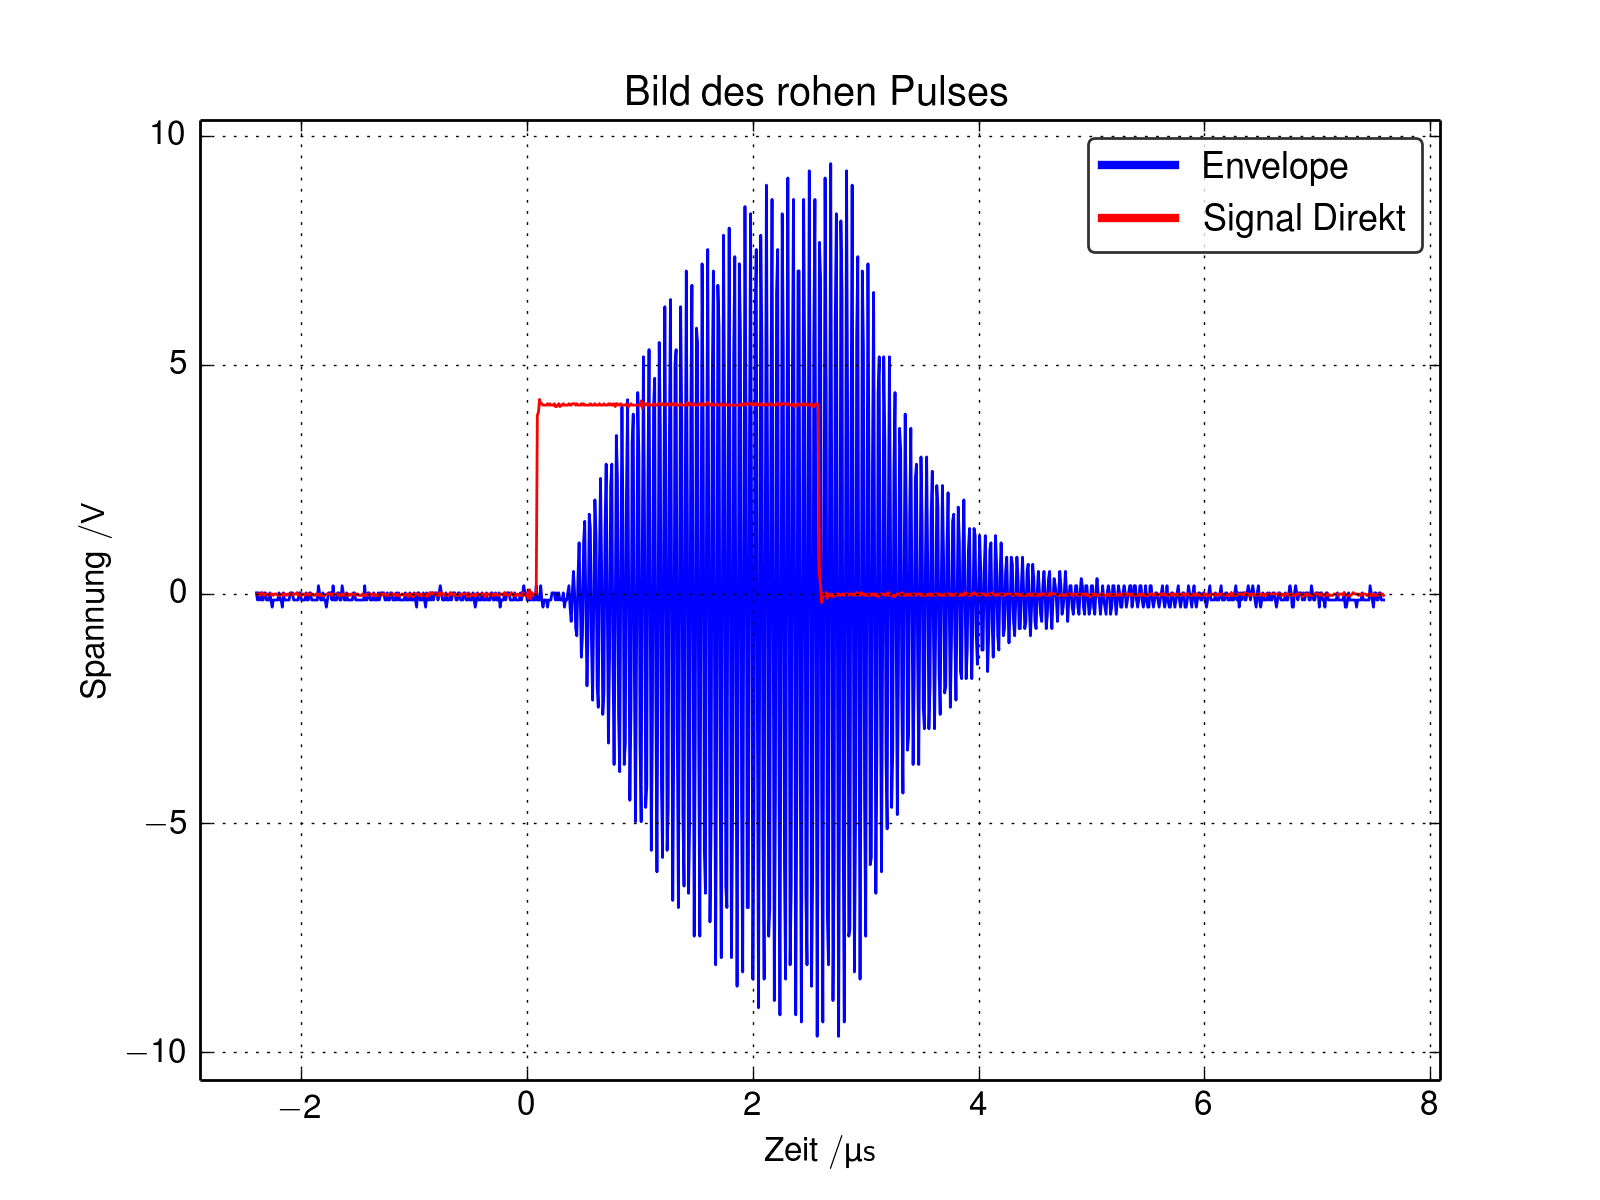
\includegraphics[width=\textwidth]{Figures/RohPuls1.png}
        \caption{Signal des elektromagnetischen Pulses.
          Sowohl direkt am Ausgang des Synthesizer als auch an der Probe
          gemessen.}
        \label{figRohPuls}
      \end{figure}

      
    \end{section}
    %%%%%%%%%%%%%%%%%%%%%%%%%%%%%
    
  \end{chapter}
  %%%%%%%%%%%%%%%%%%%%
  
  
  \newpage
  %%%%%%%%%%%%%%%%%%%%
  %%%%%%%%%%%%%%%%%%%%
  %%%%%%%%%%%%%%%%%%%%
  \begin{chapter}{Durchführung und Auswertung der Messdaten}
    \label{chp:Auswertung}
    
    Nachdem nun alles nach Anleitung aufgebaut und verkabelt ist und das Signal
    optimiert wurde, beginnen wir nun mit den eigentlichen Messungen dieses
    Versuches.
    
    %%%%%%%%%%%%%%%%%%%%%%%%%%%%%%
    %%%%%%%%%%%%%%%%%%%%%%%%%%%%%%
    %%%%%%%%%%%%%%%%%%%%%%%%%%%%%%
    \begin{section}{Offset der Spannungen}
      \label{chpOffset}
      
      Zunächst führen wir eine Messung ohne jegliches Signal durch um einen
      möglichen \textit{Offset} zu bestimmen.
      Dazu schalten wir die Messspannungen für \textit{Envelope}, \textit{Q} und
      \textit{I} am Oszilloskop ein, lassen aber das Signal am Synthesizer
      ausgeschaltet.
      \begin{figure}[hb]
        \centering
        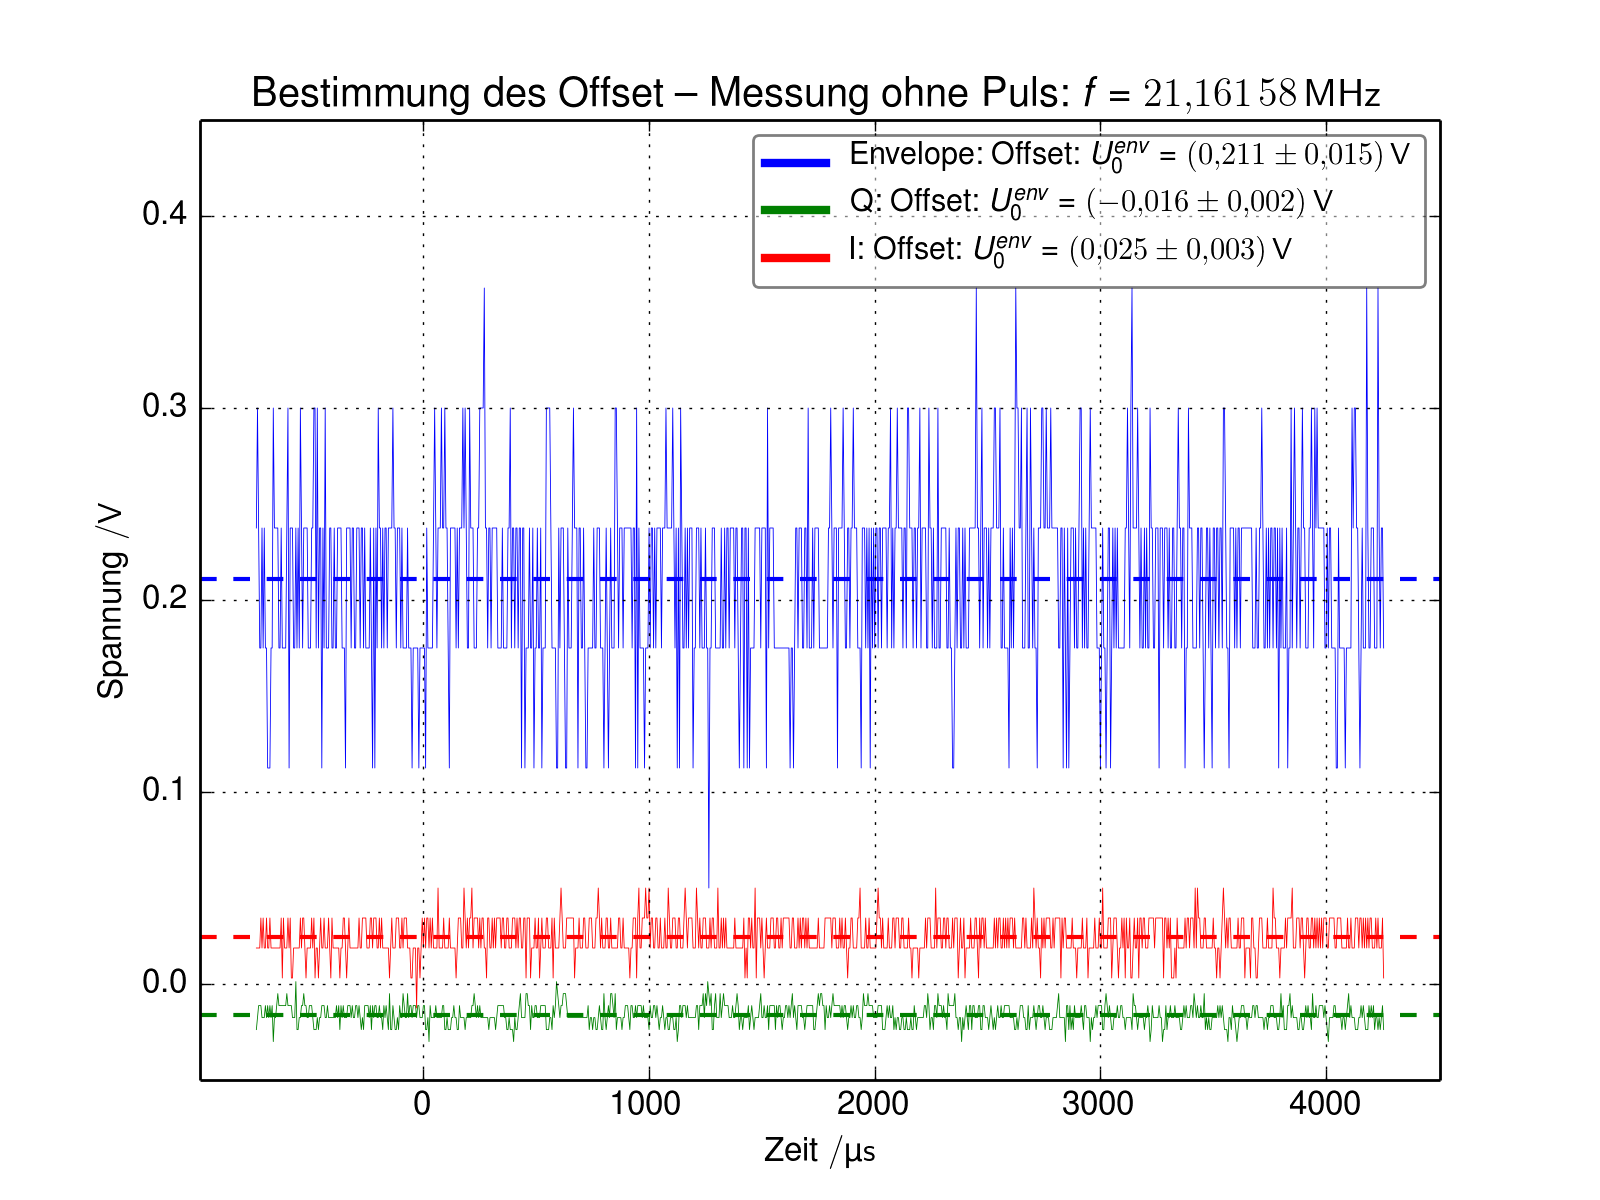
\includegraphics[width=\textwidth]{Figures/Offset.png}
        \caption{Messdaten \textbf{ohne} eingeschalteten Puls zur
          \textit{Offset}--Messung.}
        \label{figOffset}
      \end{figure}
      
      Die von uns damit gemessenen Spannungen sind in \cref{figOffset} zusammen
      mit den berechneten Mittelwerten dargestellt.
      Alle hiernach genommenen Messwerte haben wir mit den gefundenen
      Offsets korrigiert.
      
      \todo{Bild wirklich hier rein oder lieber im anhang?}
      
    \end{section}
    %%%%%%%%%%%%%%%%%%%%%%%%%%%%%
    
    
    
    %%%%%%%%%%%%%%%%%%%%%%%%%%%%%%
    %%%%%%%%%%%%%%%%%%%%%%%%%%%%%%
    %%%%%%%%%%%%%%%%%%%%%%%%%%%%%%
    \begin{section}[Free Induction Decay]{
        \underline{F}ree \underline{I}nduction \underline{D}ecay}
      \label{chpFID}
      
      Als nächstes optimieren wir das FID--Signal indem wir die Gradienten
      des Magnetfeldes so verstellen, dass das Profil möglichst einem
      exponentiellem Abfall entspricht.
      Da wir das Profil über das Oszilloskop nur nach Augenmaß einstellen
      konnten, entspricht das Profil leider nicht perfekt dem angestrebten
      exponentiellen Verlauf.
      Im Zeitraum von etwa $\SI{1.5}{\milli\second}$ bis
      $\SI{4.5}{\milli\second}$ konnten wir dennoch ein ausreichend
      gutes exponentielles Profil erreichen.
      An diesen zeitlichen Bereich passen wir \cref{eqFID}
      \begin{equation}
        \label{eqFID}
        M(\tau)=M_{0}\exp{\left(-\frac{\tau}{T_{2}^{*}}+c\right)},
      \end{equation}
      mit einer Versatzvariablen $c$ um den leicht verschobenen exponentiellen
      Abfall zu kompensieren, an.
      \Cref{figFIDenv} stellt das FID--Signal und die daran angepasste Kurve
      graphisch mit dem sowohl wir als auch unser Tutor einigermaßen zufrieden
      waren dar.
      
      Zu beginn des Versuches haben wir eine Resonanz der Lamorfrequenz von
      $\SI{21.16158}{\mega\hertz}$ gefunden.
      Da sich im laufe des Versuches etwas am FID--Profil verändert hat
      mussten wir nach einiger Zeit die Frequenz verändern um weiterhin die
      Resonanzfrequenz zu treffen.
      Daher haben wir dazu eine Frequenz von $\SI{21.16133}{\mega\hertz}$
      eingestellt.
      Bei welcher Frequenz eine Messung aufgenommen wurde ist jeweils im Titel
      der Graphiken festgehalten.
      
      \begin{figure}[htb]
        \centering
        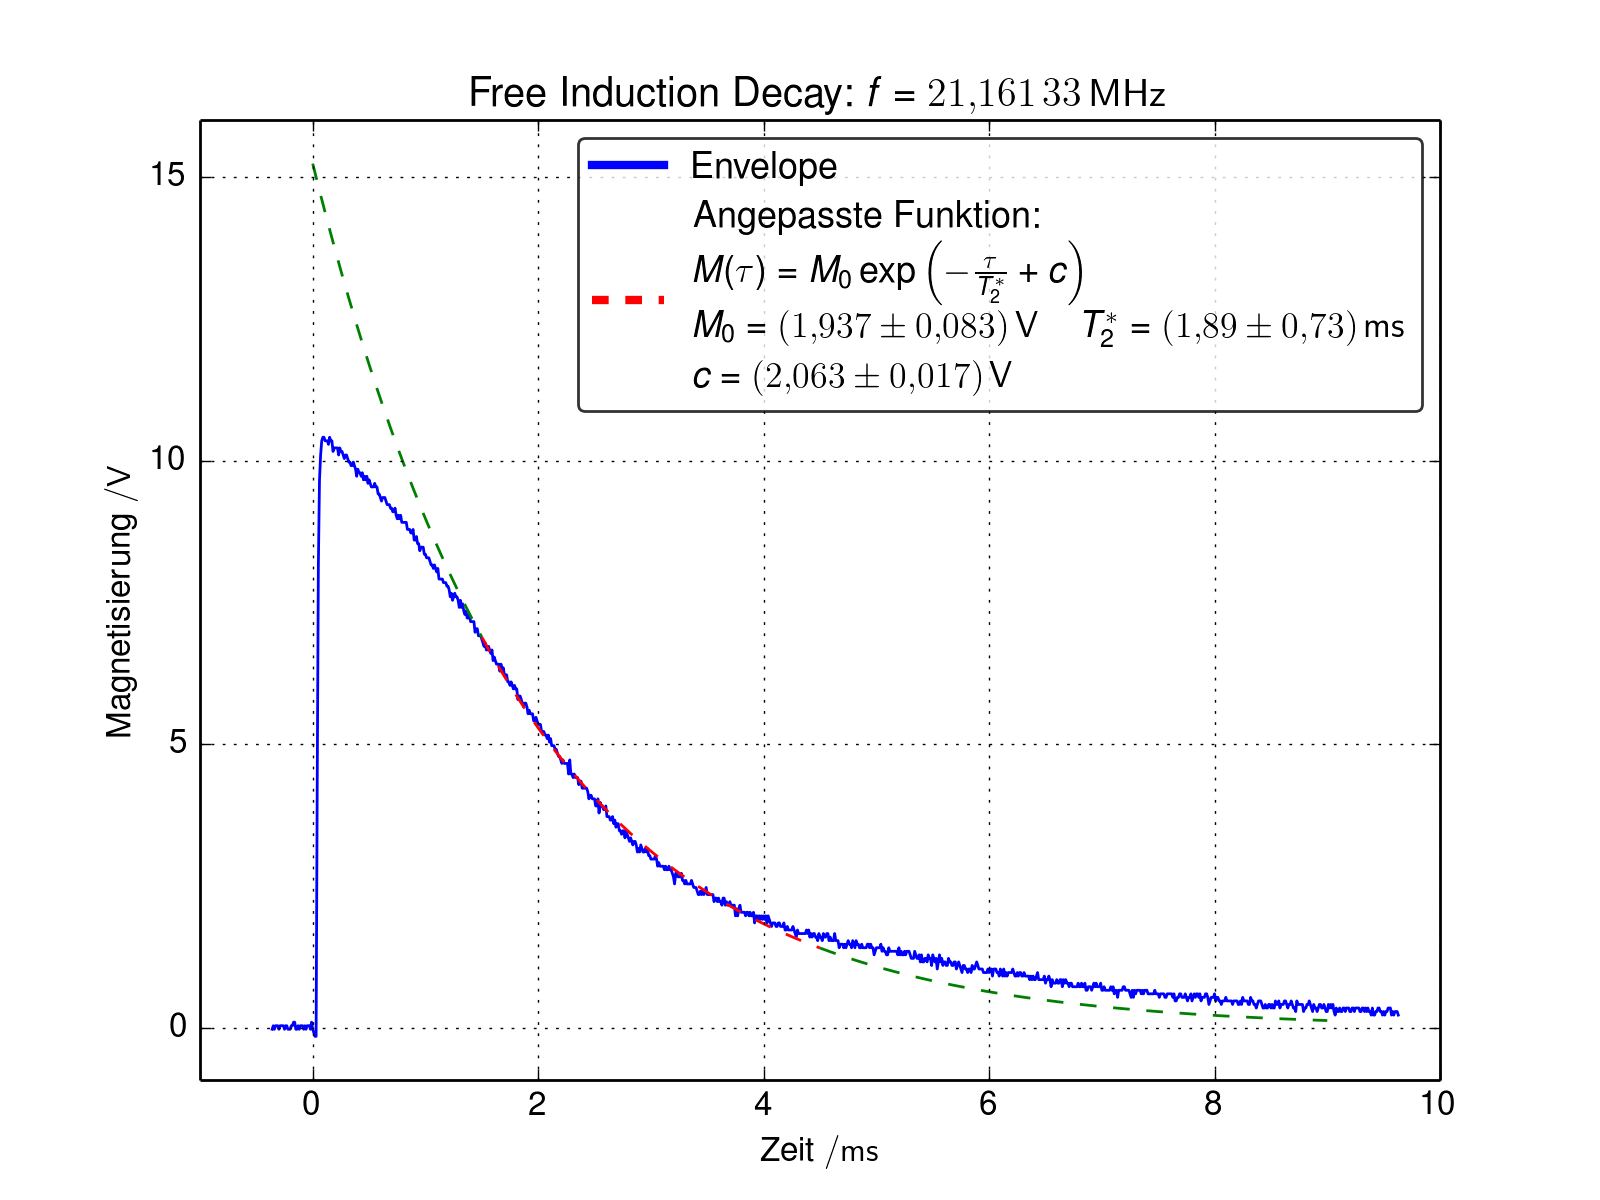
\includegraphics[width=\textwidth]{Figures/FID_env2.png}
        \caption{\textit{Free Induction Decay} Antwort--Signal und angepasste
          Zerfalls--Funktion.}
        \label{figFIDenv}
      \end{figure}
      
      \todo{fehlt noch was zu T2*. und ist das HIER tatsächlich richtig
        oder besser nachher wenn T2* tatsächlich gebraucht wird?}
      
%       \begin{figure}[htb]
%         \centering
%         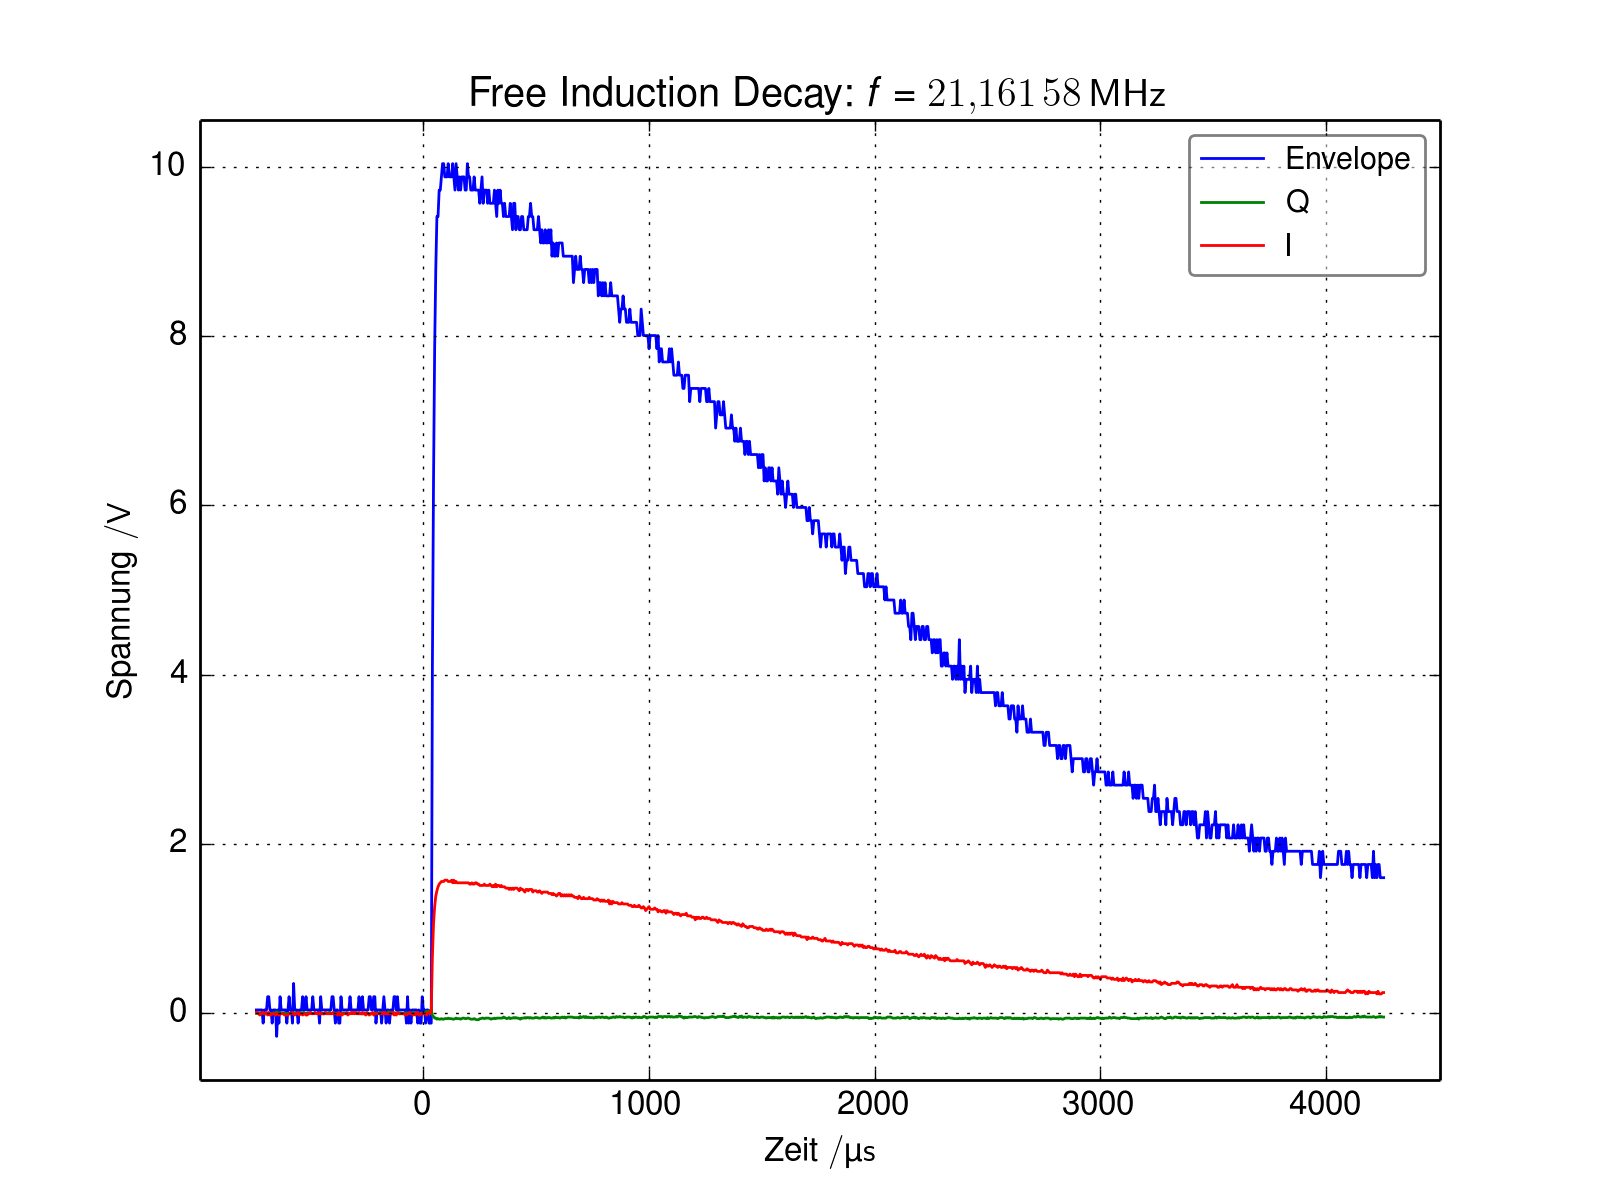
\includegraphics[width=\textwidth]{Figures/FID_env_Q_I0.png}
%         \caption{\textit{Free Induction Decay} Signal gemessen an der Probe.
%           Zusammen mit \textit{Q}-- und \textit{I}--Signal.}
%         \label{figFIDenvQI}
%       \end{figure}
      
    \end{section}
    %%%%%%%%%%%%%%%%%%%%%%%%%%%%%
    
    
    
    %%%%%%%%%%%%%%%%%%%%%%%%%%%%%%
    %%%%%%%%%%%%%%%%%%%%%%%%%%%%%%
    %%%%%%%%%%%%%%%%%%%%%%%%%%%%%%
    \begin{section}{Justierung der Pulszeiten}
      \label{chpPulszeiten}
      
      Um heraus zu finden welche Pulslängen einem $\pi$--, bzw.\
      $\frac{\pi}{2}$--Puls entsprechen, messen wir Amplitude des
      Antwort--Signales während wir die Pulslänge variieren.
      Zunächst bestimmen wir den $\pi$--Puls, indem wir eine Pulsdauer suchen,
      bei der das Antwort--Signal eine minimale Amplitude besitzt.
      Bei dieser Pulslänge löschen sich Puls und Antwort--Signal komplett aus.
      \todo{Warum?}
      Für unseren Aufbau haben wir hierbei eine Länge des $\pi$--Pulses von
      $A_{len}=\SI{5.44}{\micro\second}$ gefunden.
      Für den $\frac{\pi}{2}$--Puls gilt, dass dieser genau der halben Länge
      des $\pi$--Pulses, also $A_{len}=\SI{2.72}{\micro\second}$, entspricht.
      
      \todo{Fertig?}
      \todo{oder ist das schon im aufbau gemacht worden?}
      
    \end{section}
    %%%%%%%%%%%%%%%%%%%%%%%%%%%%%
    
    
    
    %%%%%%%%%%%%%%%%%%%%%%%%%%%%%%
    %%%%%%%%%%%%%%%%%%%%%%%%%%%%%%
    %%%%%%%%%%%%%%%%%%%%%%%%%%%%%%
    \begin{section}{Rabi--Oszillation}
      \label{chpRabi}
      
      Um die Rabi--Oszillation zu messen, benutzen wir einen Puls und variieren
      dessen Länge.
      Dabei messen wir die maximale Amplitude des Antwort--Signales und des
      In--Phase Signales der Probe für jede eingestellte Pulslänge.
      Diese Messung wiederholen wir für eine leicht andere Frequenz.
      \todo{warum?}
      Um den Verlauf der Oszillation besser zu erkennen haben wir eine
      Betragsfunktion des Sinus angepasst und zusammen mit den Messdaten in
      \cref{figRabifreq12} abgebildet.
      
      Wie wir auch schon in der Theorie erwartet haben steigt die Amplitude
      des Antwort--Signales mit an sobald sich die Pulslänge dem
      $\frac{\pi}{2}$--Puls nähert und dort ein Maximum annimmt.
      Für eine Pulslänge um die des $\pi$--Pulses nimmt die Amplitude wieder
      ab um dann bei der Länge entsprechend eines $\frac{3\pi}{4}$--Pulses
      wieder ein Maximum erreicht.
      Das In--Phase Signal...
      \todo{haben wir bei den unteren Oszillationen ein vorzeichen übersehen
        oder soll das auch ein sinus betrag sein? Martin hat da eine normale
        sinus schwingung!}
      
      
%       \begin{figure}[htb]
%         \centering
%         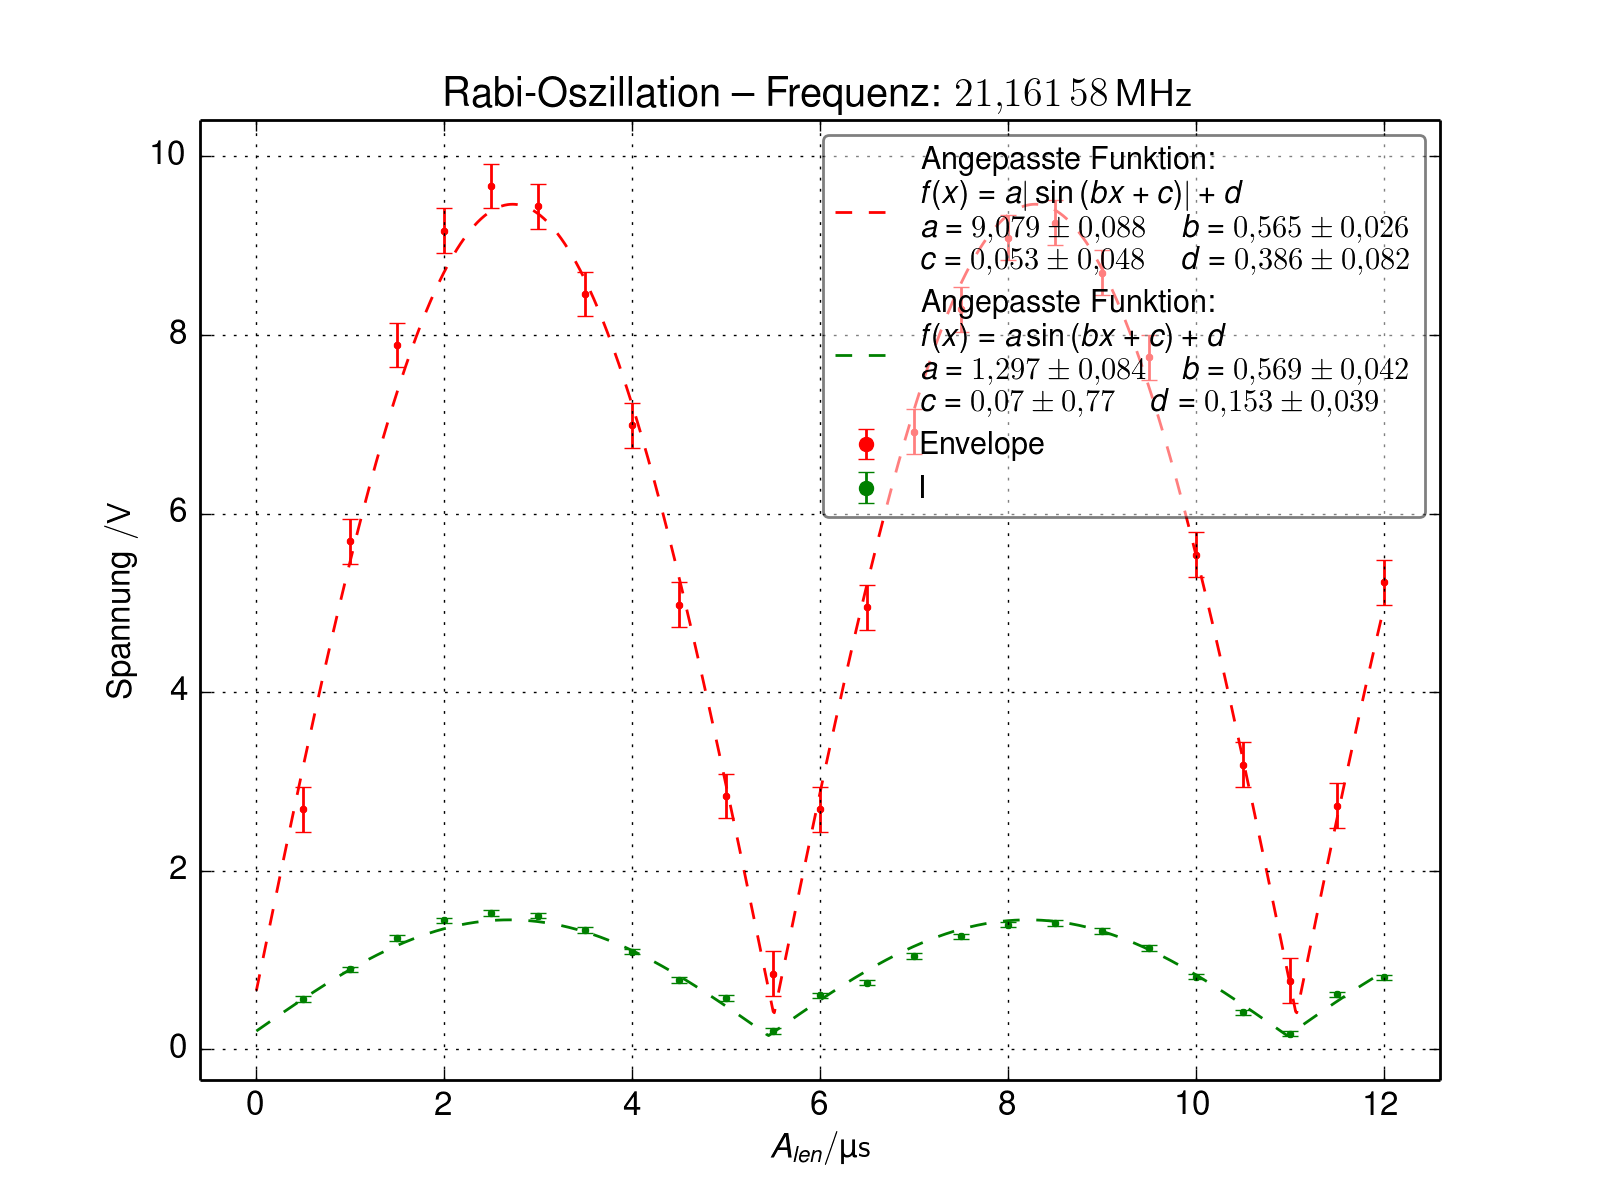
\includegraphics[width=\textwidth]{Figures/Rabi_freq1.png}
%         \caption{bla bla.}
%         \label{figRabifreq1}
%       \end{figure}
%       
%       \begin{figure}[htb]
%         \centering
%         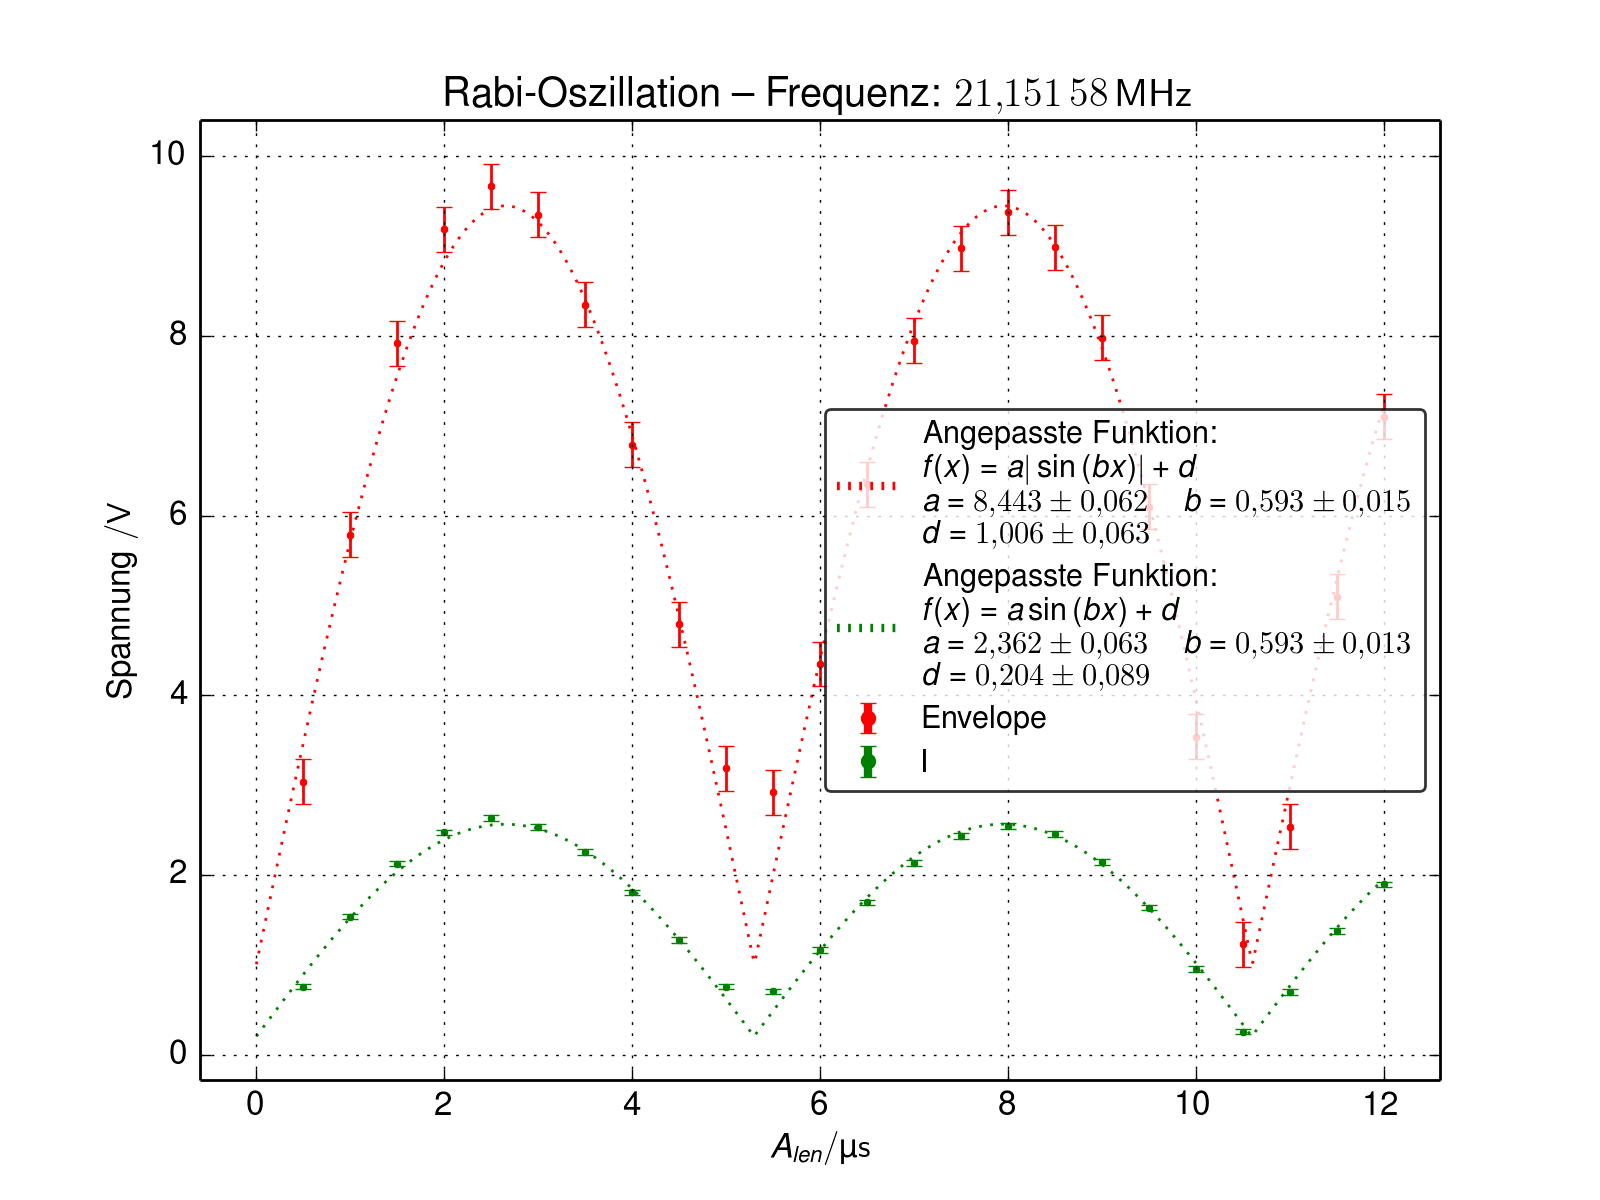
\includegraphics[width=\textwidth]{Figures/Rabi_freq2.png}
%         \caption{bla bla.}
%         \label{figRabifreq2}
%       \end{figure}
      
      \begin{figure}[htb]
        \centering
        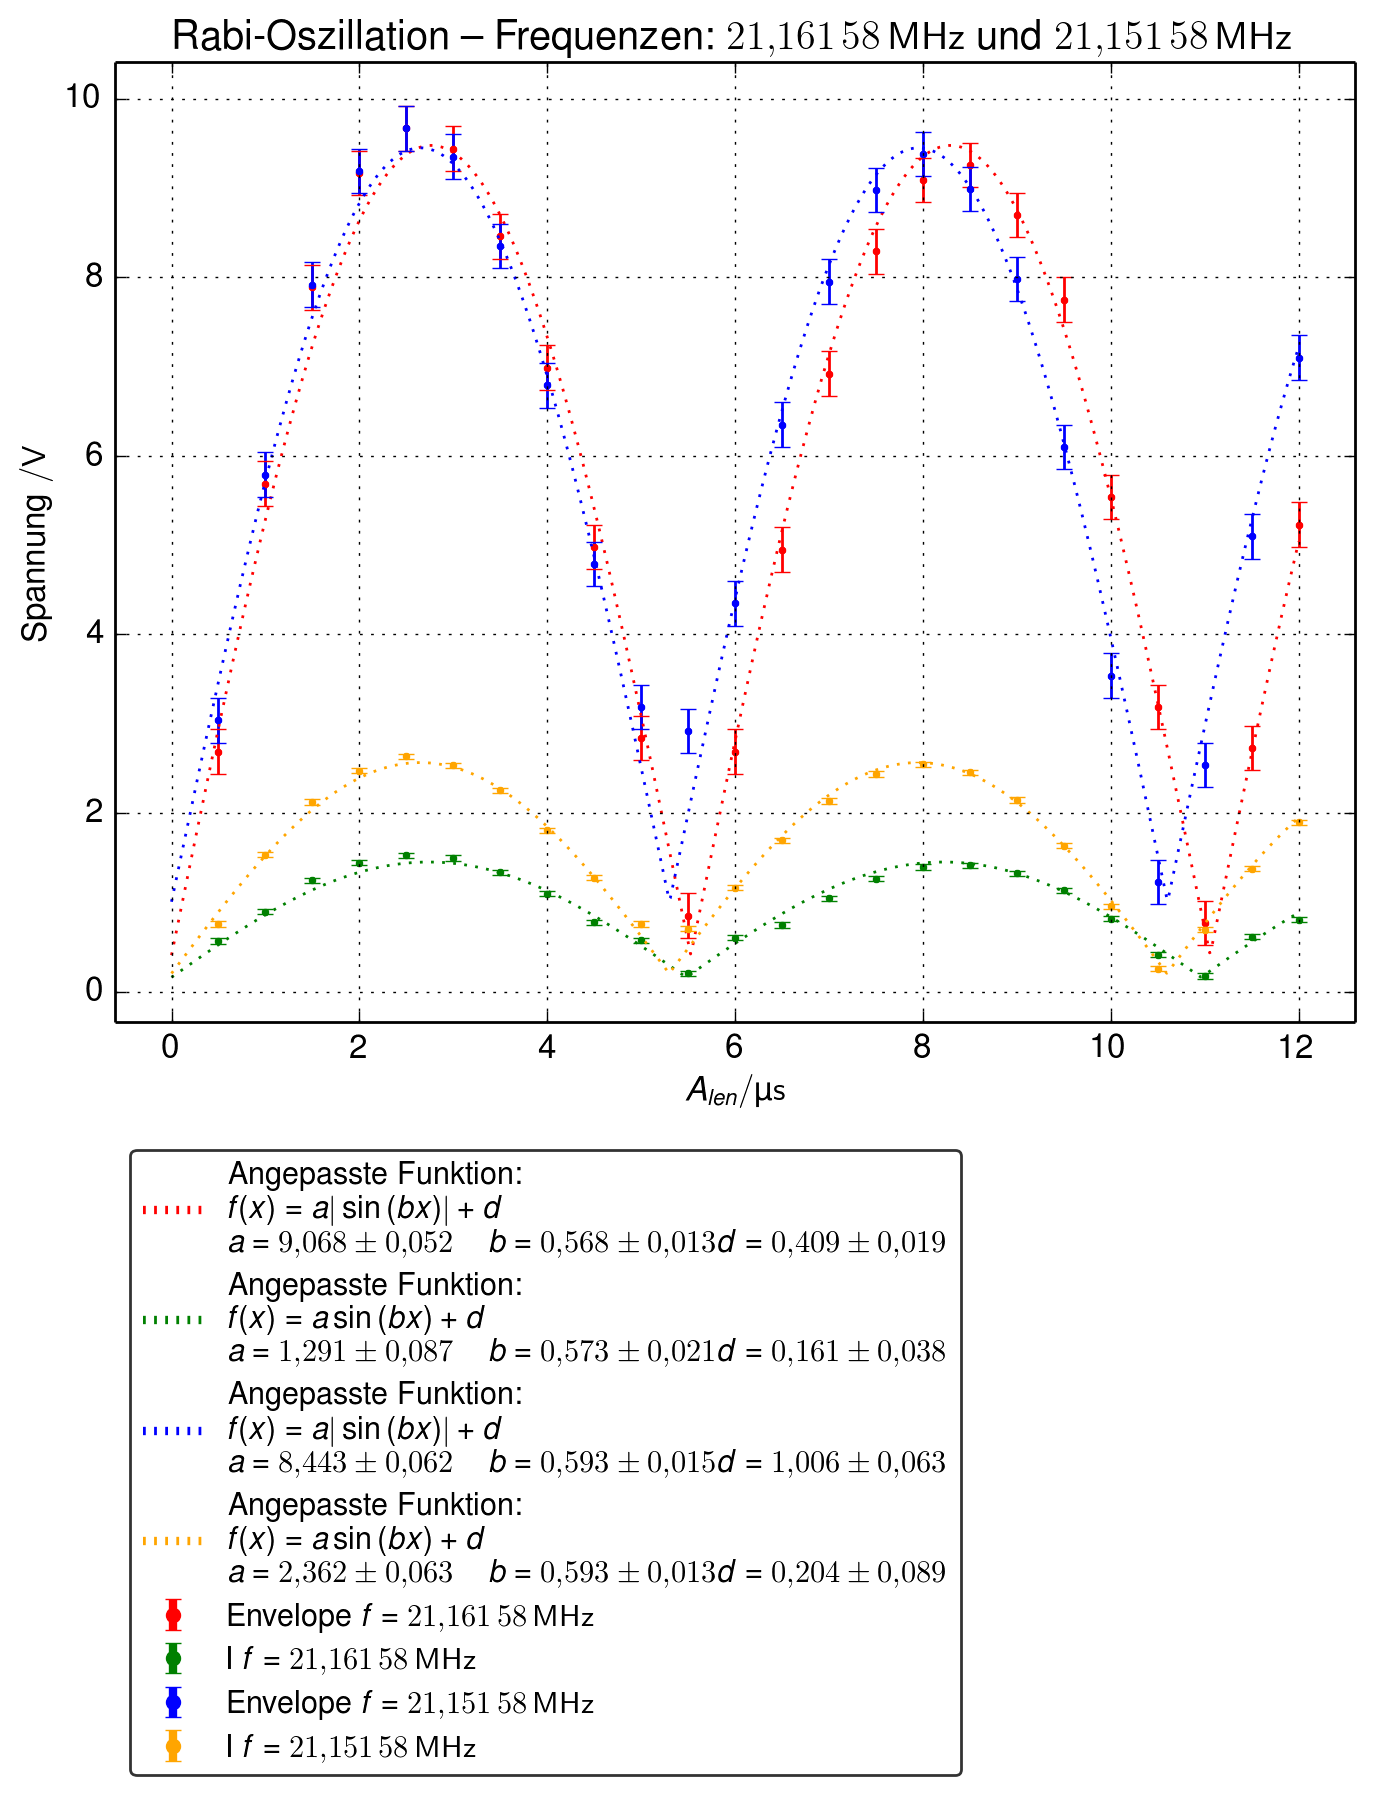
\includegraphics[width=.9\textwidth]{Figures/Rabi_freq12.png}
        \caption{bla bla.}
        \label{figRabifreq12}
      \end{figure}
      
      \todo{Alle Bilder wirklich hier rein oder lieber im anhang?}
      
    \end{section}
    %%%%%%%%%%%%%%%%%%%%%%%%%%%%%
    
    
    
    %%%%%%%%%%%%%%%%%%%%%%%%%%%%%%
    %%%%%%%%%%%%%%%%%%%%%%%%%%%%%%
    %%%%%%%%%%%%%%%%%%%%%%%%%%%%%%
    \begin{section}[Longitudinale Relaxationszeit]{
        Longitudinale Relaxationszeit $T_{1}$}
      \label{chpLongRelax}
      
      %%%%%%%%%%%%%%%%%%%%%%%%%%%%%%%%%%%%%%%
      %%%%%%%%%%%%%%%%%%%%%%%%%%%%%%%%%%%%%%%
      %%%%%%%%%%%%%%%%%%%%%%%%%%%%%%%%%%%%%%%
      \begin{subsection}{Sättigungs--Zurückgewinnung}
        \label{chpLongRelaxSaettigung}
        
        
        
        
        \begin{figure}[htb]
          \centering
          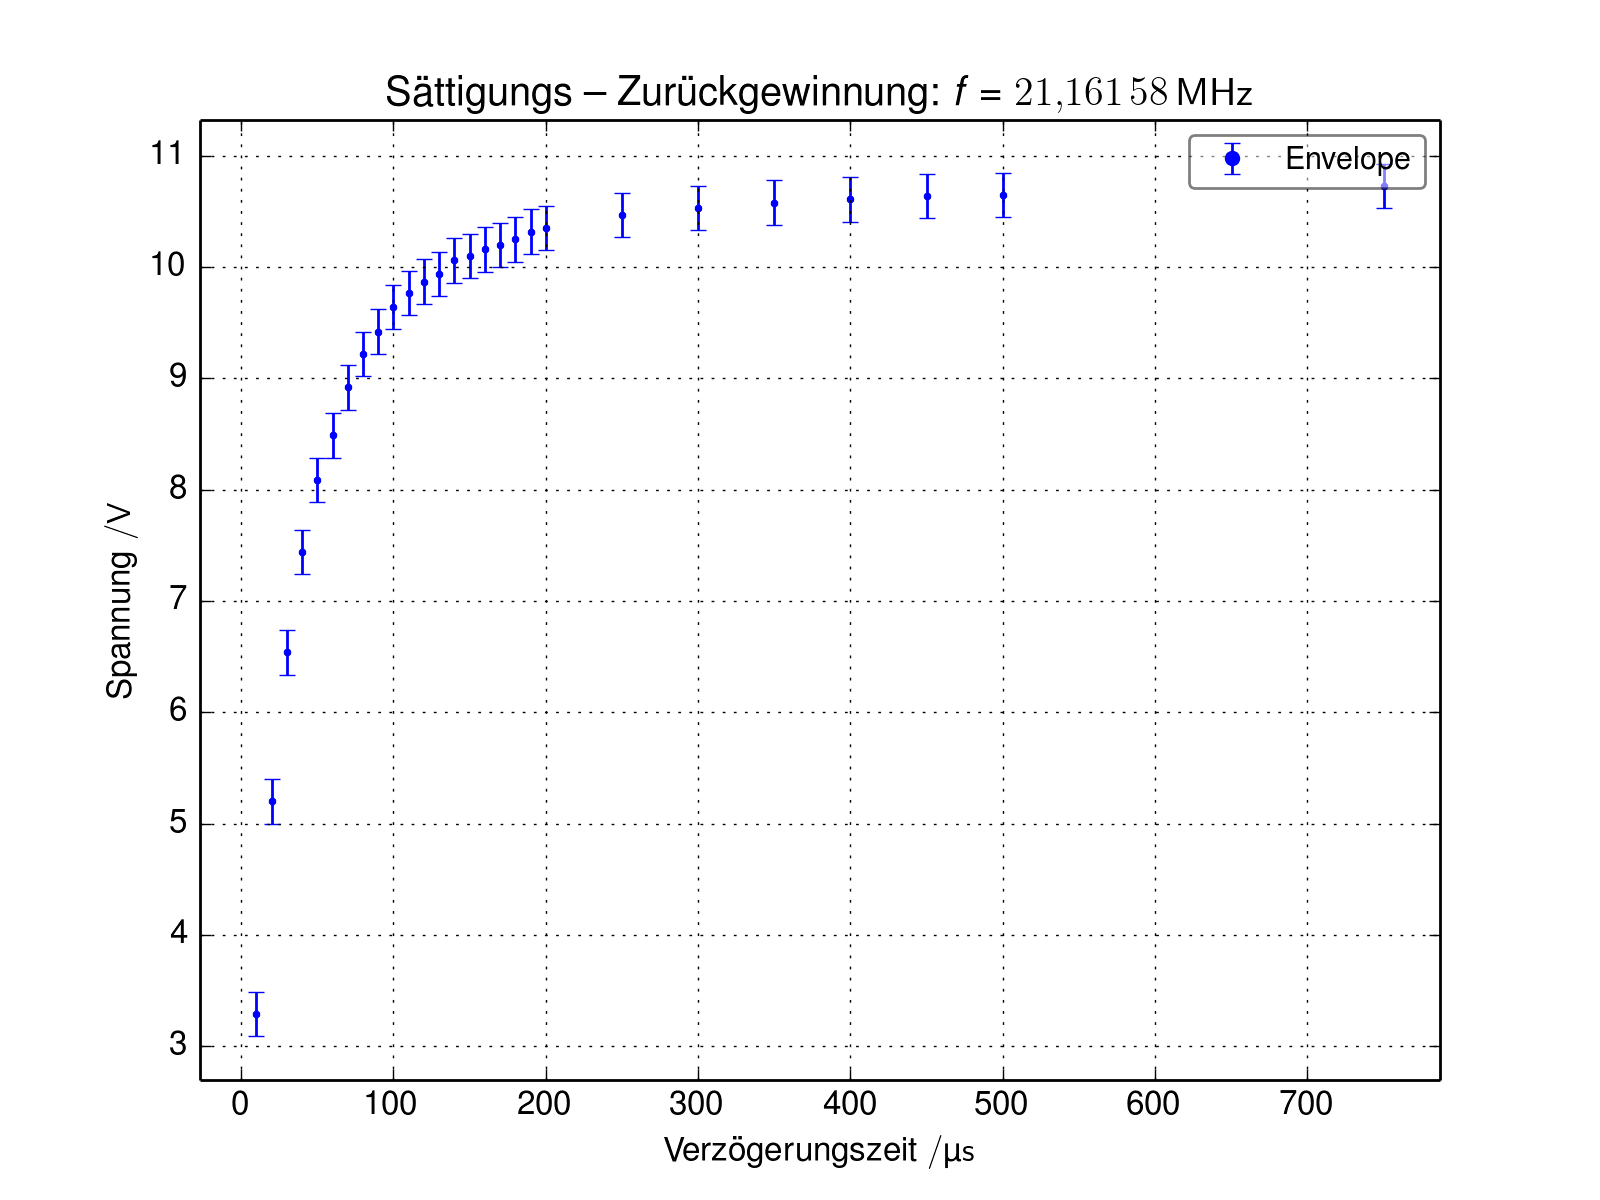
\includegraphics[width=\textwidth]
          {Figures/SaettigungsZurueckgewinnung.png}
          \caption{bla bla.}
          \label{figSaettigung}
        \end{figure}
        
        
      \end{subsection}
      %%%%%%%%%%%%%%%%%%%%%%%%%%%%%%%%%%%%%%%
      
      
      \newpage
      %%%%%%%%%%%%%%%%%%%%%%%%%%%%%%%%%%%%%%%
      %%%%%%%%%%%%%%%%%%%%%%%%%%%%%%%%%%%%%%%
      %%%%%%%%%%%%%%%%%%%%%%%%%%%%%%%%%%%%%%%
      \begin{subsection}{Polarisations--Zurückgewinnung}
        \label{chpLongRelaxPolarisation}
        
        
        
        
        \begin{figure}[htb]
          \centering
          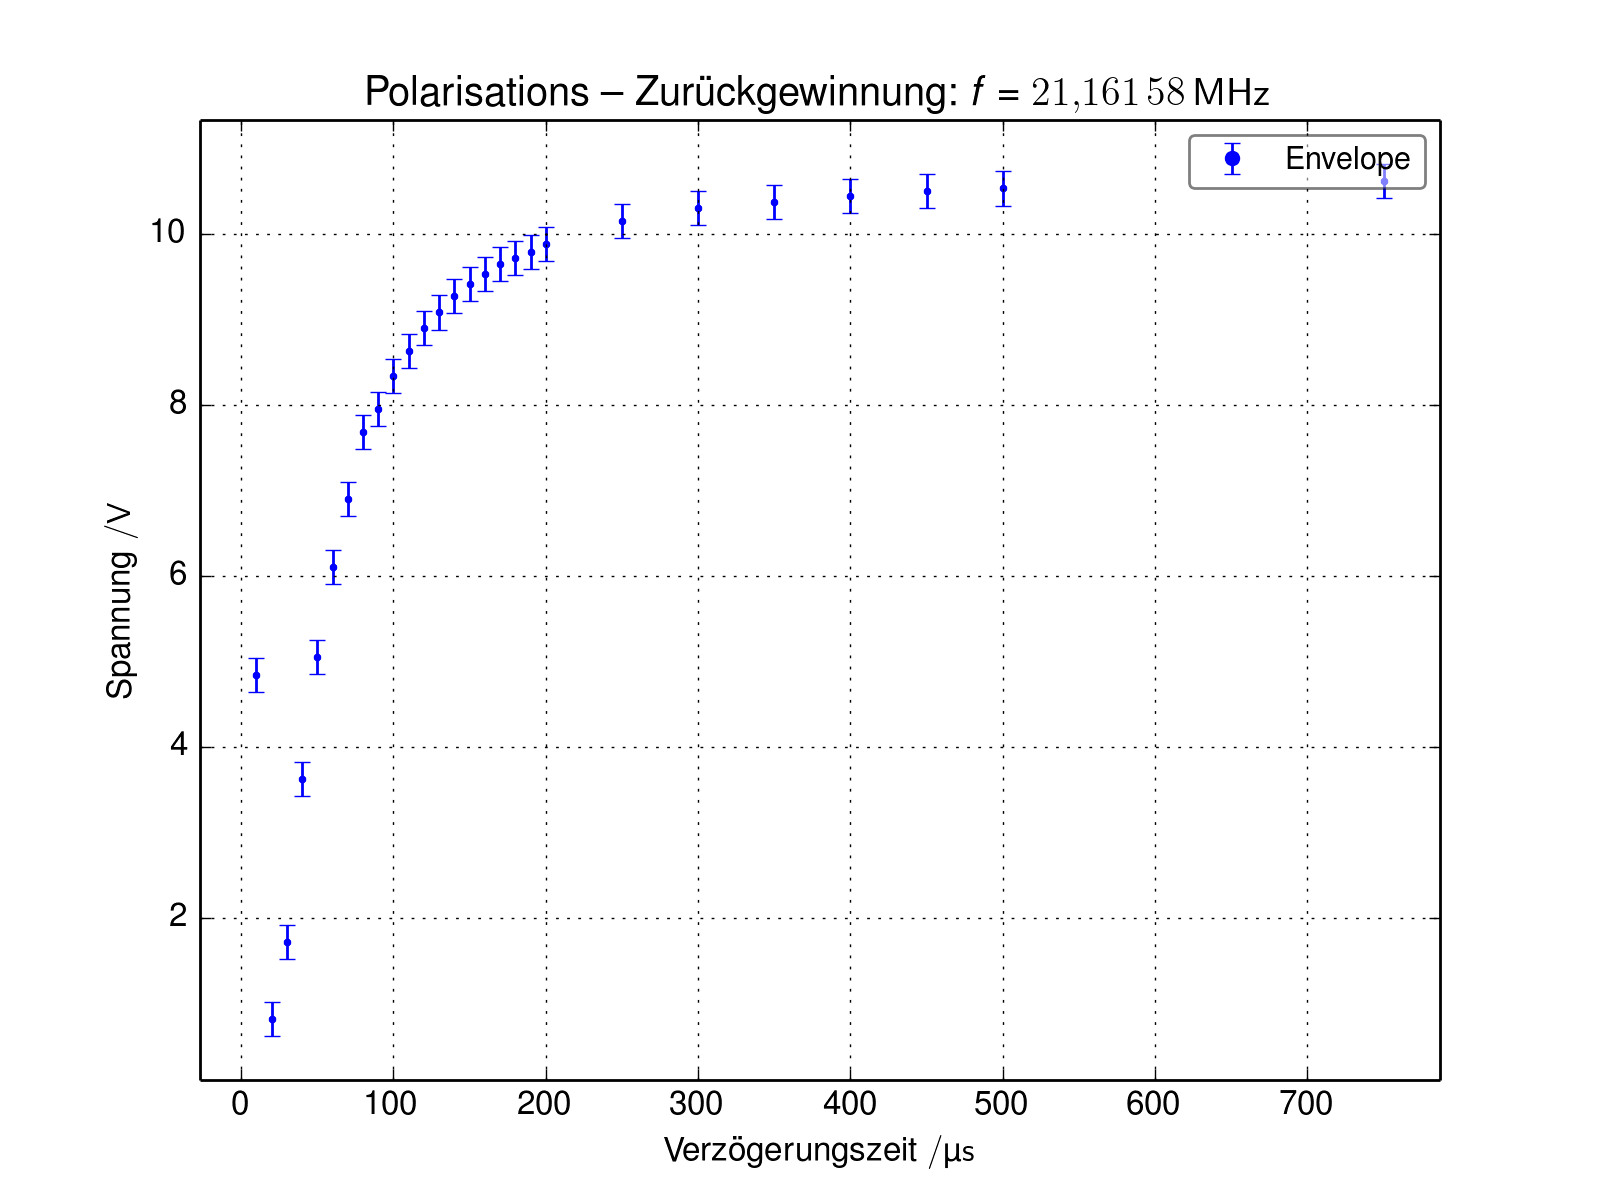
\includegraphics[width=\textwidth]
          {Figures/PolarisationsZurueckgewinnung.png}
          \caption{bla bla.}
          \label{figPolarisation}
        \end{figure}
        
        
      \end{subsection}
      %%%%%%%%%%%%%%%%%%%%%%%%%%%%%%%%%%%%%%%
      
    \end{section}
    %%%%%%%%%%%%%%%%%%%%%%%%%%%%%
    
    
    \newpage
    %%%%%%%%%%%%%%%%%%%%%%%%%%%%%%
    %%%%%%%%%%%%%%%%%%%%%%%%%%%%%%
    %%%%%%%%%%%%%%%%%%%%%%%%%%%%%%
    \begin{section}[Effektive Transversale Relaxationszeit]{
        Effektive Transversale Relaxationszeit $T_{2}^{*}$}
      \label{chpEffTransRelax}
      
      \todo{muss hier das FID zeug rein?}
      
    \end{section}
    %%%%%%%%%%%%%%%%%%%%%%%%%%%%%
    
    
    \newpage
    %%%%%%%%%%%%%%%%%%%%%%%%%%%%%%
    %%%%%%%%%%%%%%%%%%%%%%%%%%%%%%
    %%%%%%%%%%%%%%%%%%%%%%%%%%%%%%
    \begin{section}[Homogene Transversale Relaxationszeit]{
        Homogene Transversale Relaxationszeit $T_{2}$}
      \label{chpHomoTransRelax}
      
      \todo{Alle Bilder wirklich hier rein oder lieber im anhang?}
      
      %%%%%%%%%%%%%%%%%%%%%%%%%%%%%%%%%%%%%%%
      %%%%%%%%%%%%%%%%%%%%%%%%%%%%%%%%%%%%%%%
      %%%%%%%%%%%%%%%%%%%%%%%%%%%%%%%%%%%%%%%
      \begin{subsection}{Hahn-Spinecho-Sequenz}
        \label{chpHomoTransRelaxHahn}
        
        
        
        
        \begin{figure}[htb]
          \centering
          \begin{minipage}{.48\textwidth}
            \centering
            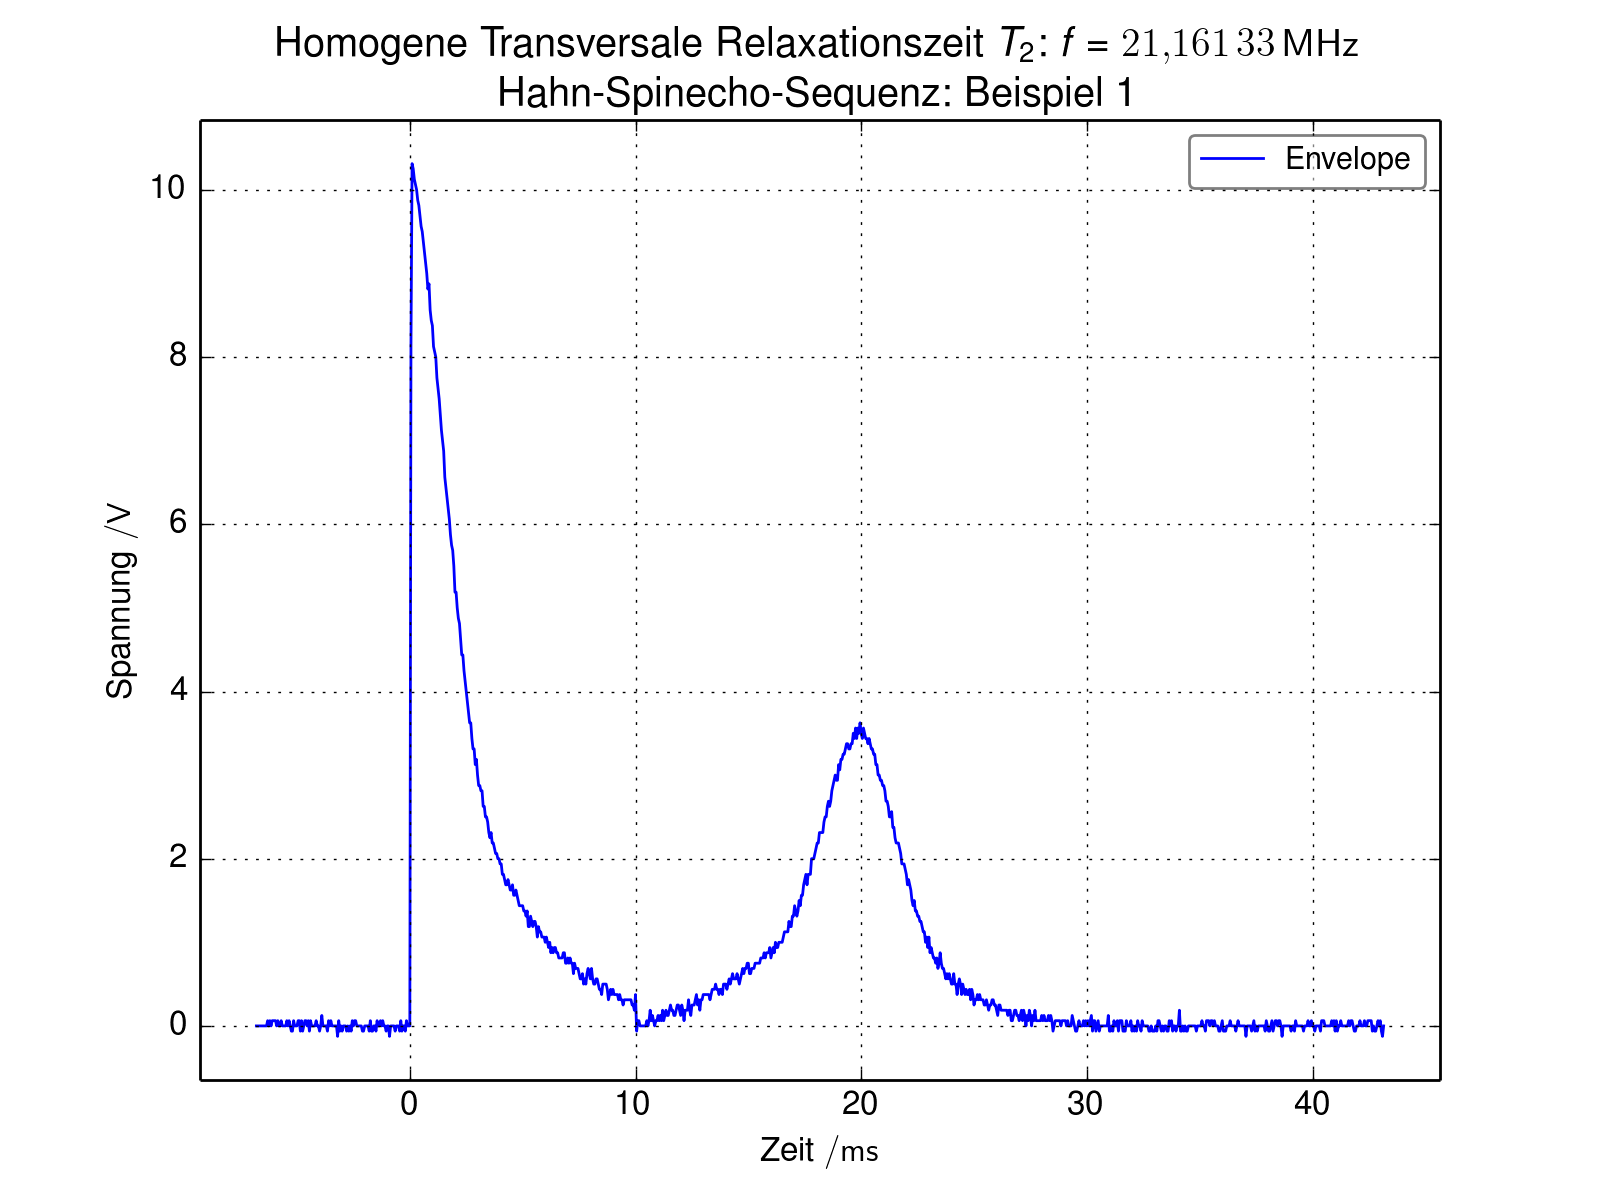
\includegraphics[width=\textwidth]
            {Figures/HomoTransRelax_Hahn_beispiel0.png}
            \caption{bla bla.}
            \label{figHahnBsp1}
          \end{minipage}\quad
          \begin{minipage}{.48\textwidth}
            \centering
            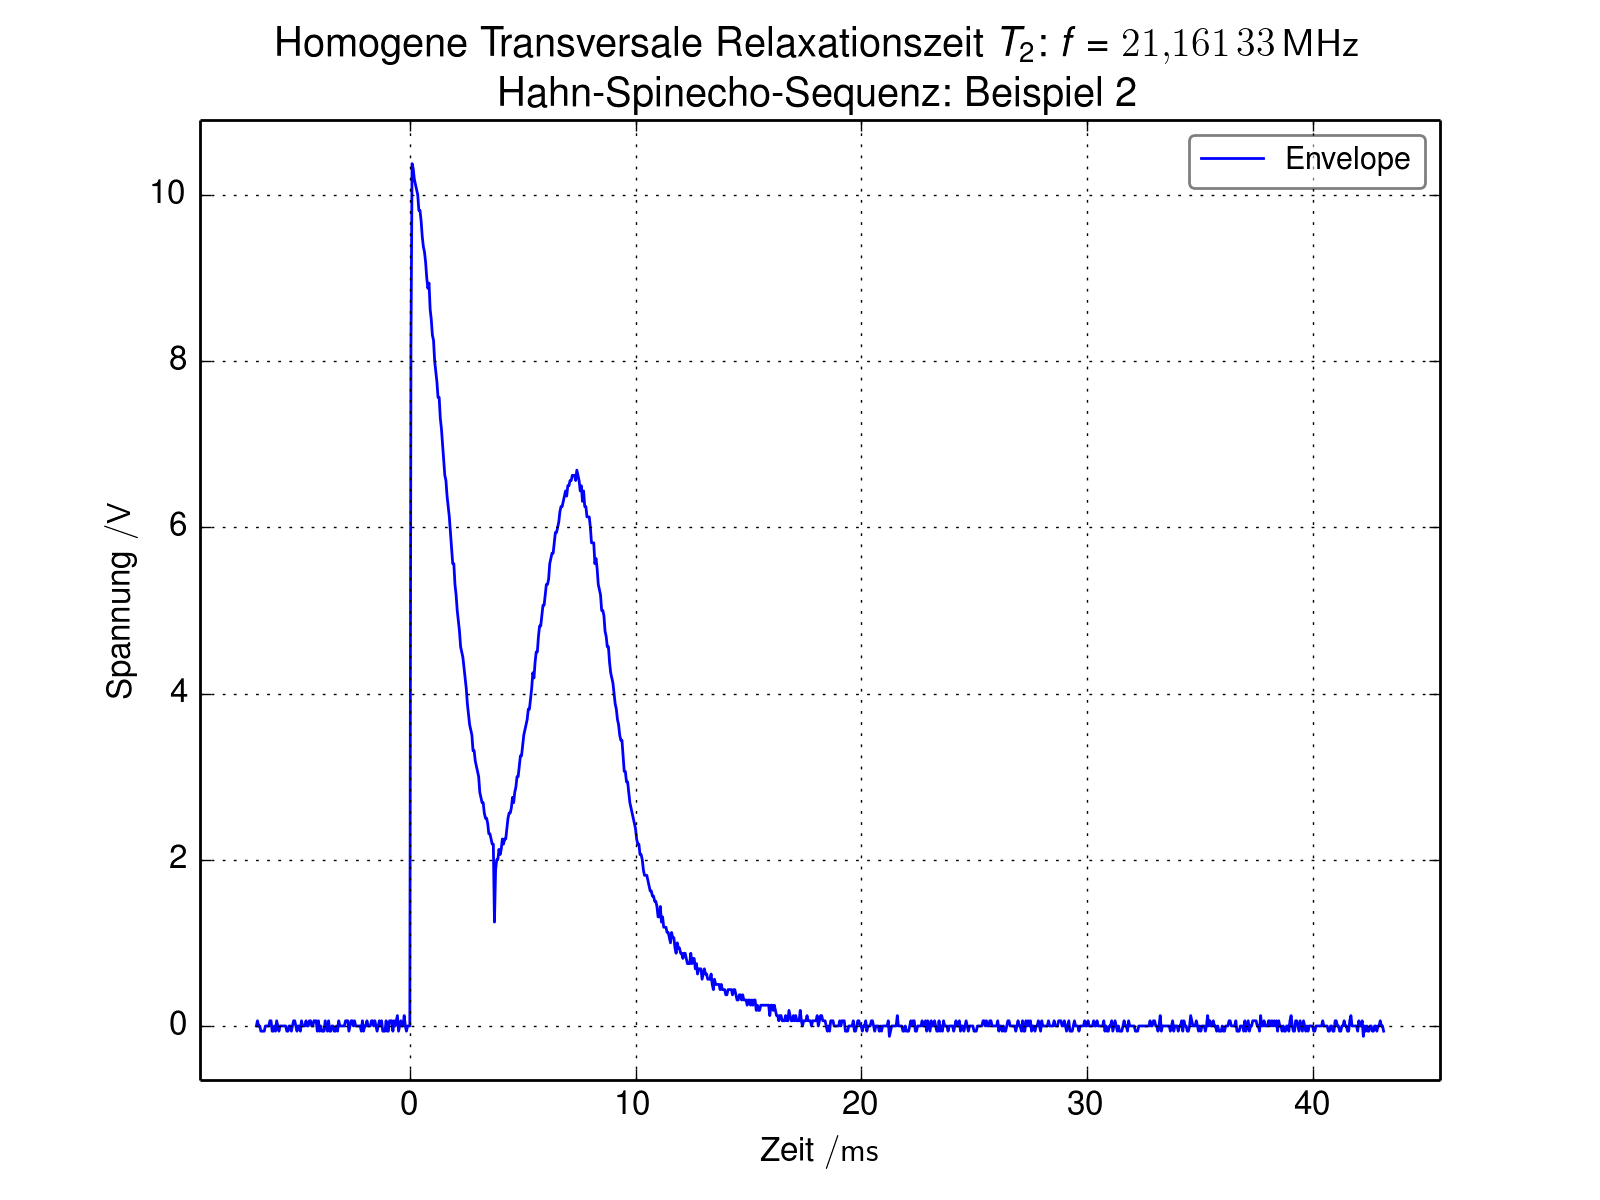
\includegraphics[width=\textwidth]
            {Figures/HomoTransRelax_Hahn_beispiel1.png}
            \caption{bla bla.}
            \label{figHahnBsp2}
          \end{minipage}
        \end{figure}
        
        
        \begin{figure}[htb]
          \centering
          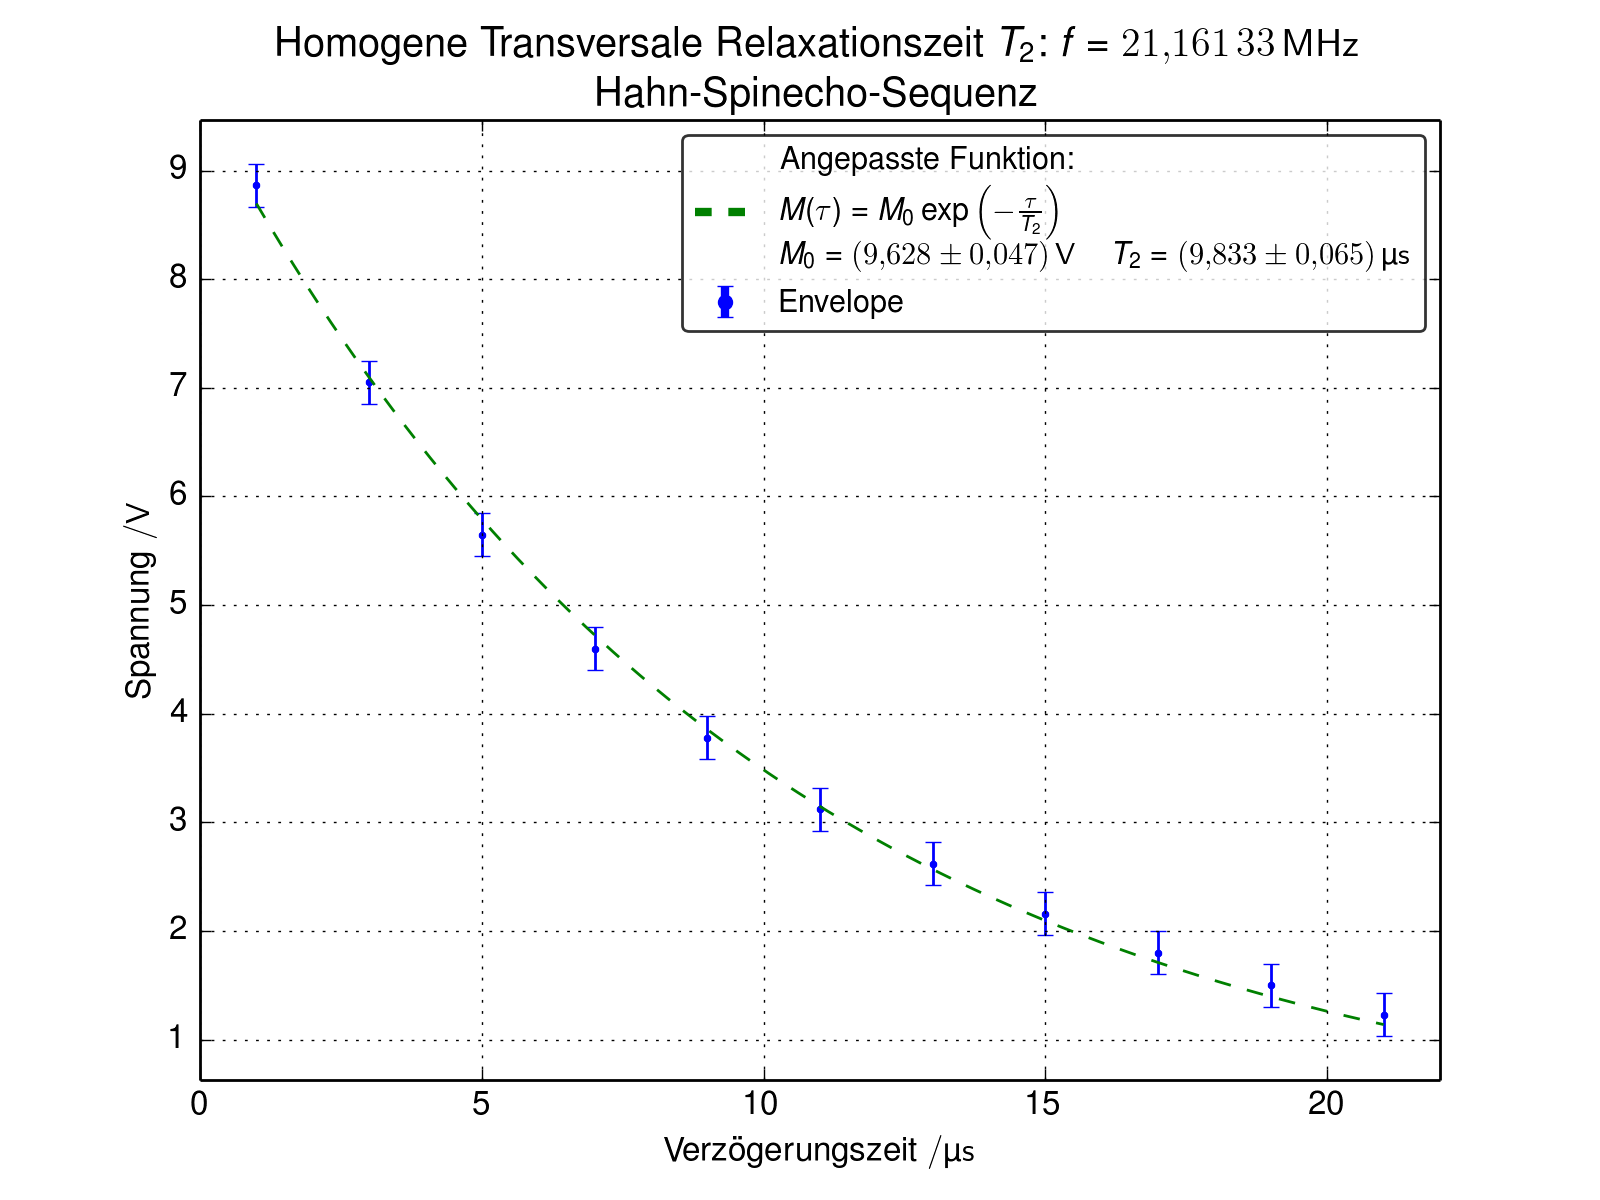
\includegraphics[width=\textwidth]
          {Figures/HomoTransRelax_Hahn.png}
          \caption{bla bla.}
          \label{figHahn}
        \end{figure}
        
        
      \end{subsection}
      %%%%%%%%%%%%%%%%%%%%%%%%%%%%%%%%%%%%%%%
      
      
      \newpage
      %%%%%%%%%%%%%%%%%%%%%%%%%%%%%%%%%%%%%%%
      %%%%%%%%%%%%%%%%%%%%%%%%%%%%%%%%%%%%%%%
      %%%%%%%%%%%%%%%%%%%%%%%%%%%%%%%%%%%%%%%
      \begin{subsection}{Carr-Purcell-Spinecho-Sequenz}
        \label{chpHomoTransRelaxCarr}
        
        
        
        
        \begin{figure}[htb]
          \centering
          \begin{minipage}{.48\textwidth}
            \centering
            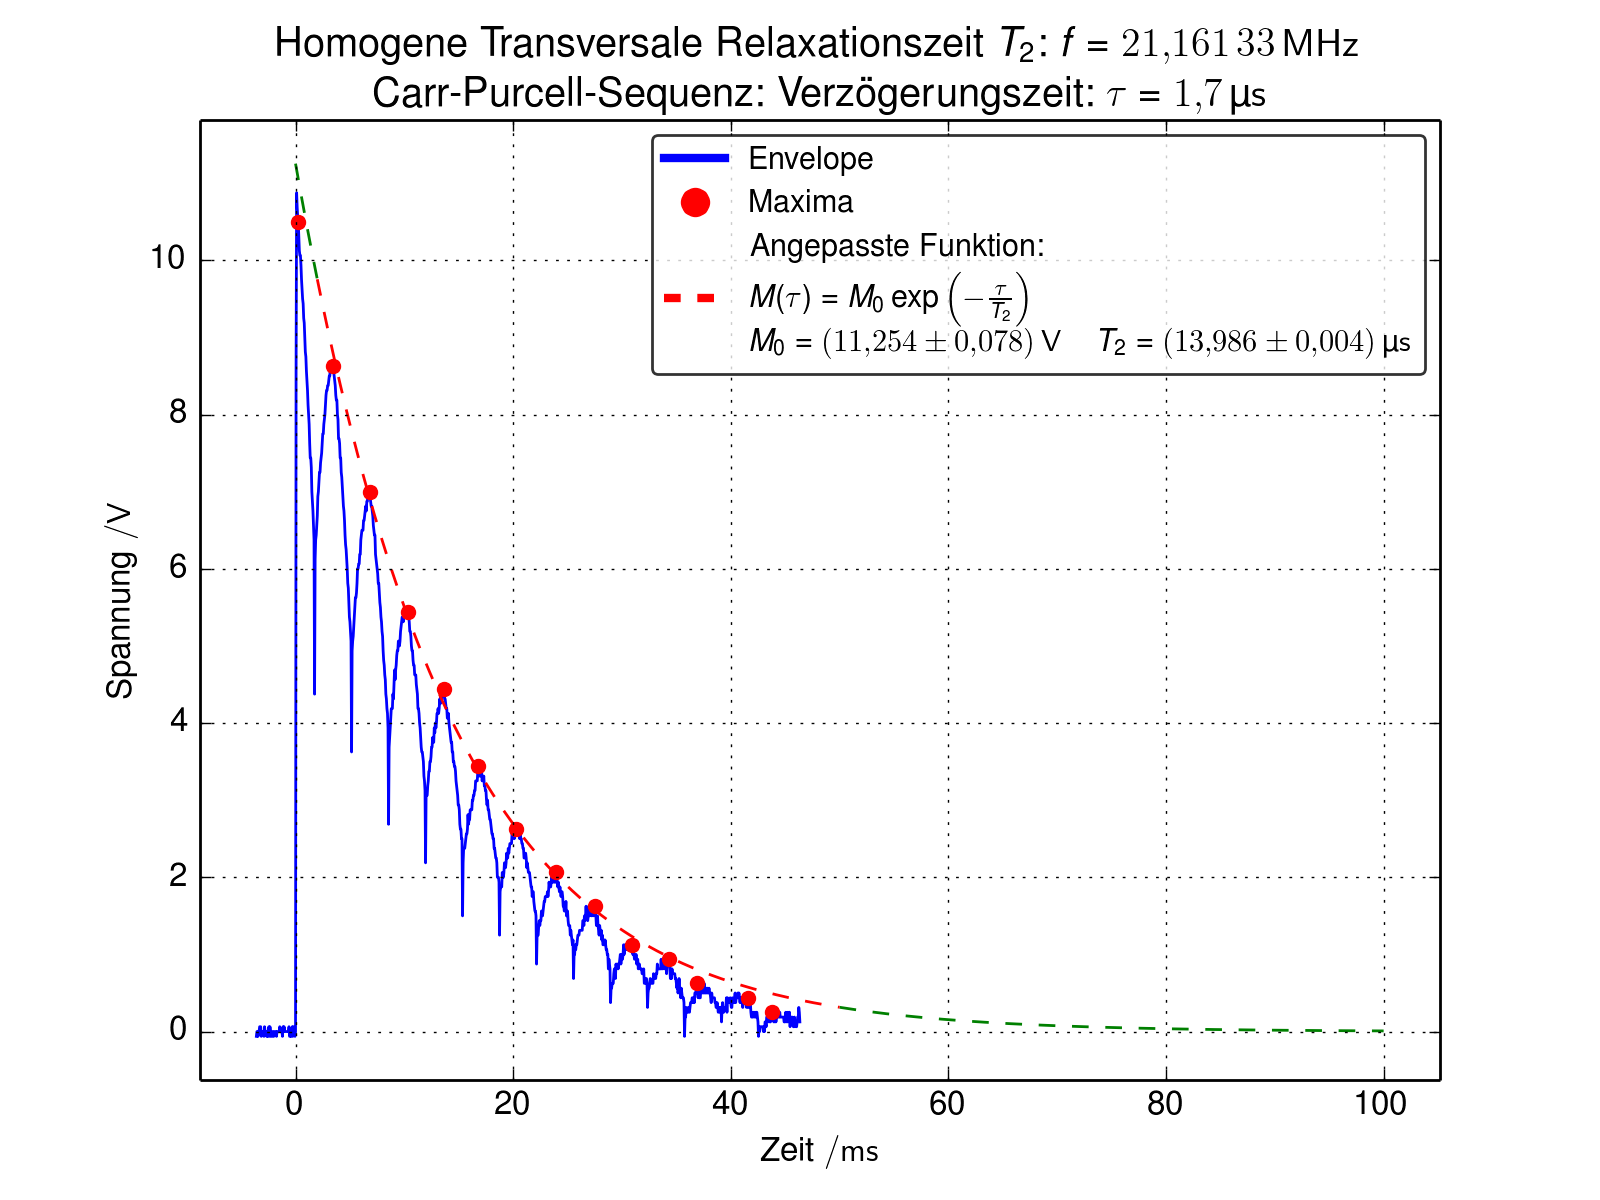
\includegraphics[width=\textwidth]
            {Figures/HomoTransRelax_Carr0.png}
            \caption{bla bla.}
            \label{figCarr0}
          \end{minipage}\\
          \begin{minipage}{.48\textwidth}
            \centering
            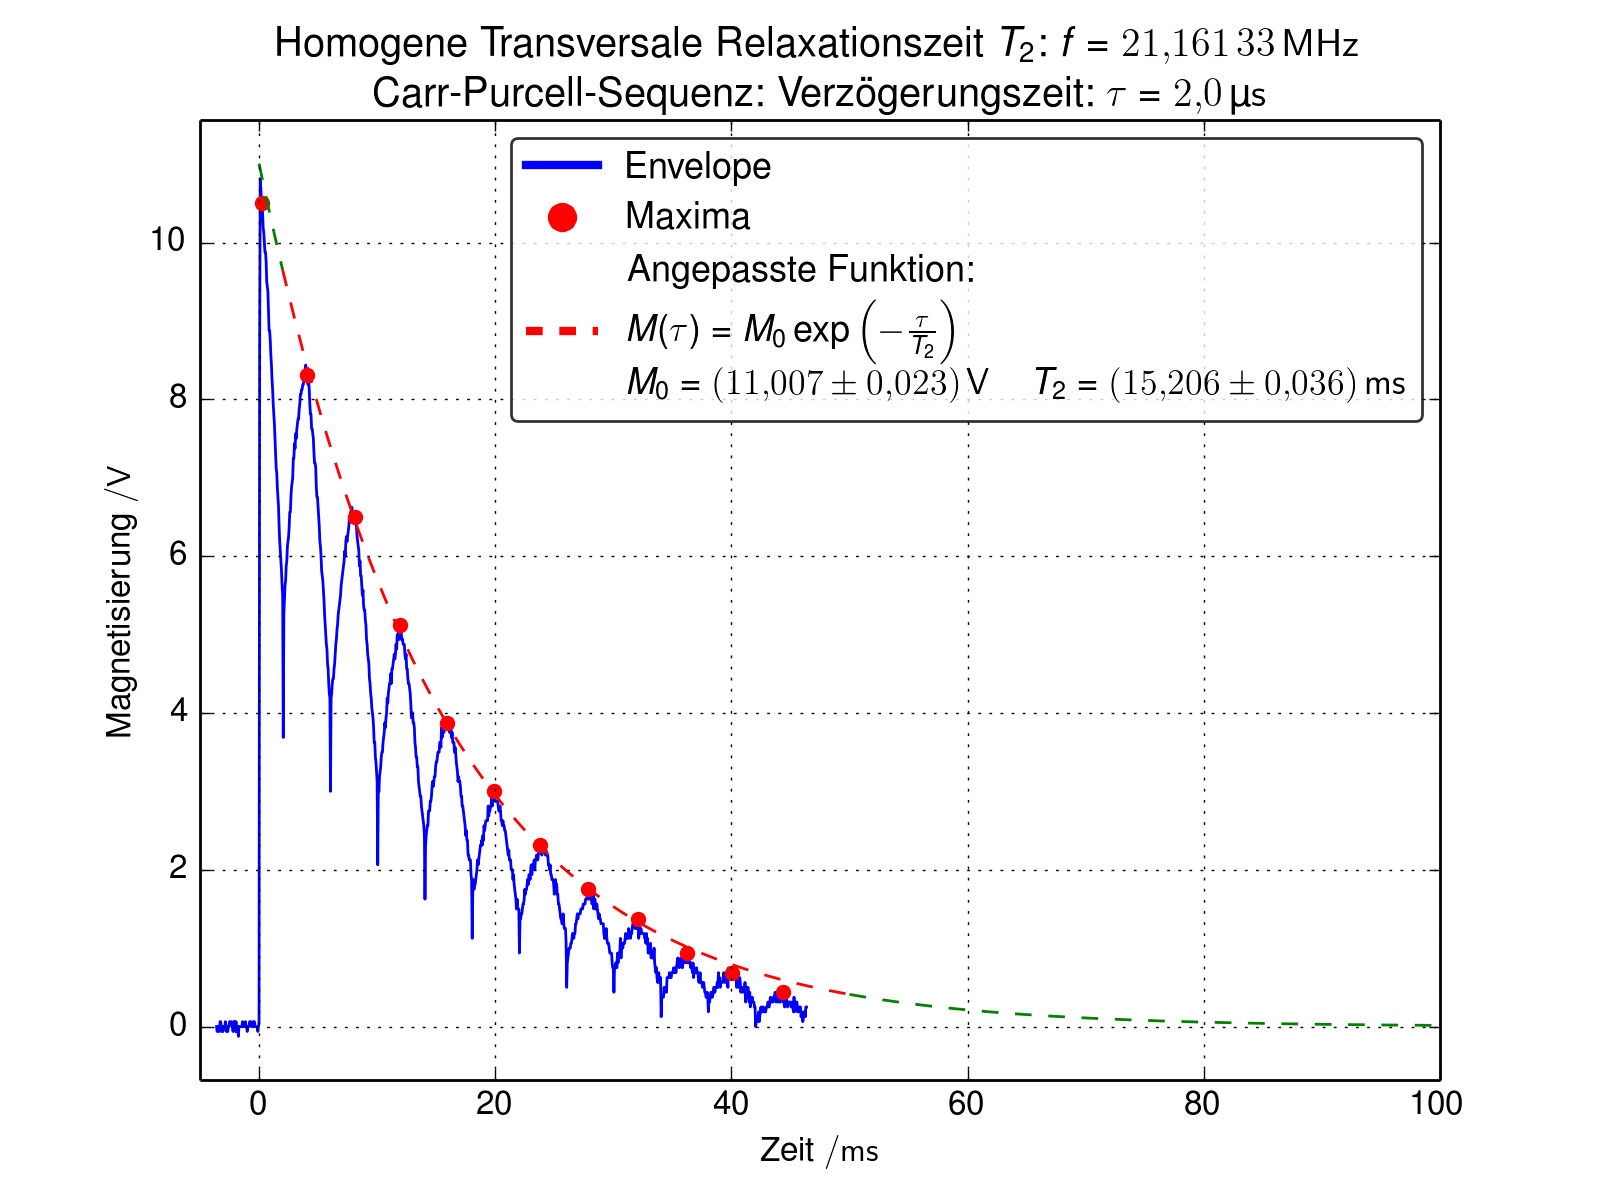
\includegraphics[width=\textwidth]
            {Figures/HomoTransRelax_Carr1.png}
            \caption{bla bla.}
            \label{figCarr1}
          \end{minipage}\quad
          \begin{minipage}{.48\textwidth}
            \centering
            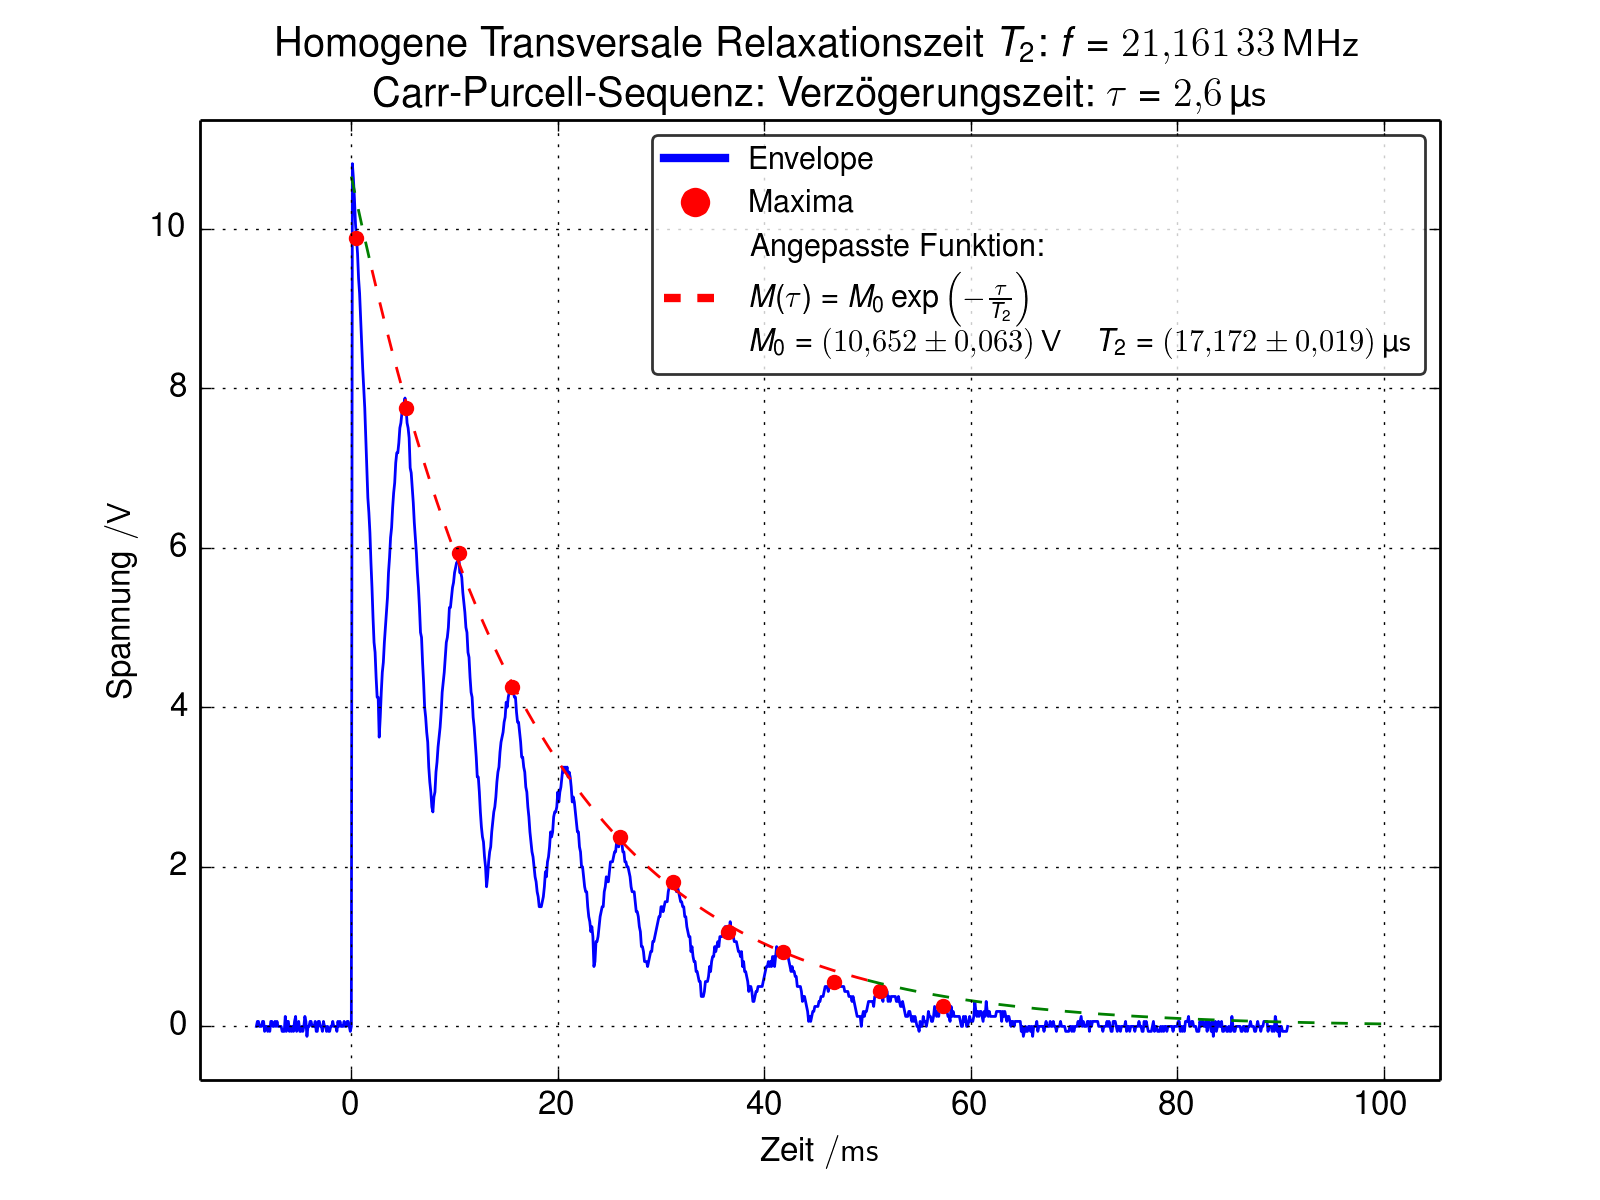
\includegraphics[width=\textwidth]
            {Figures/HomoTransRelax_Carr2.png}
            \caption{bla bla.}
            \label{figCarr2}
          \end{minipage}\\
          \begin{minipage}{.48\textwidth}
            \centering
            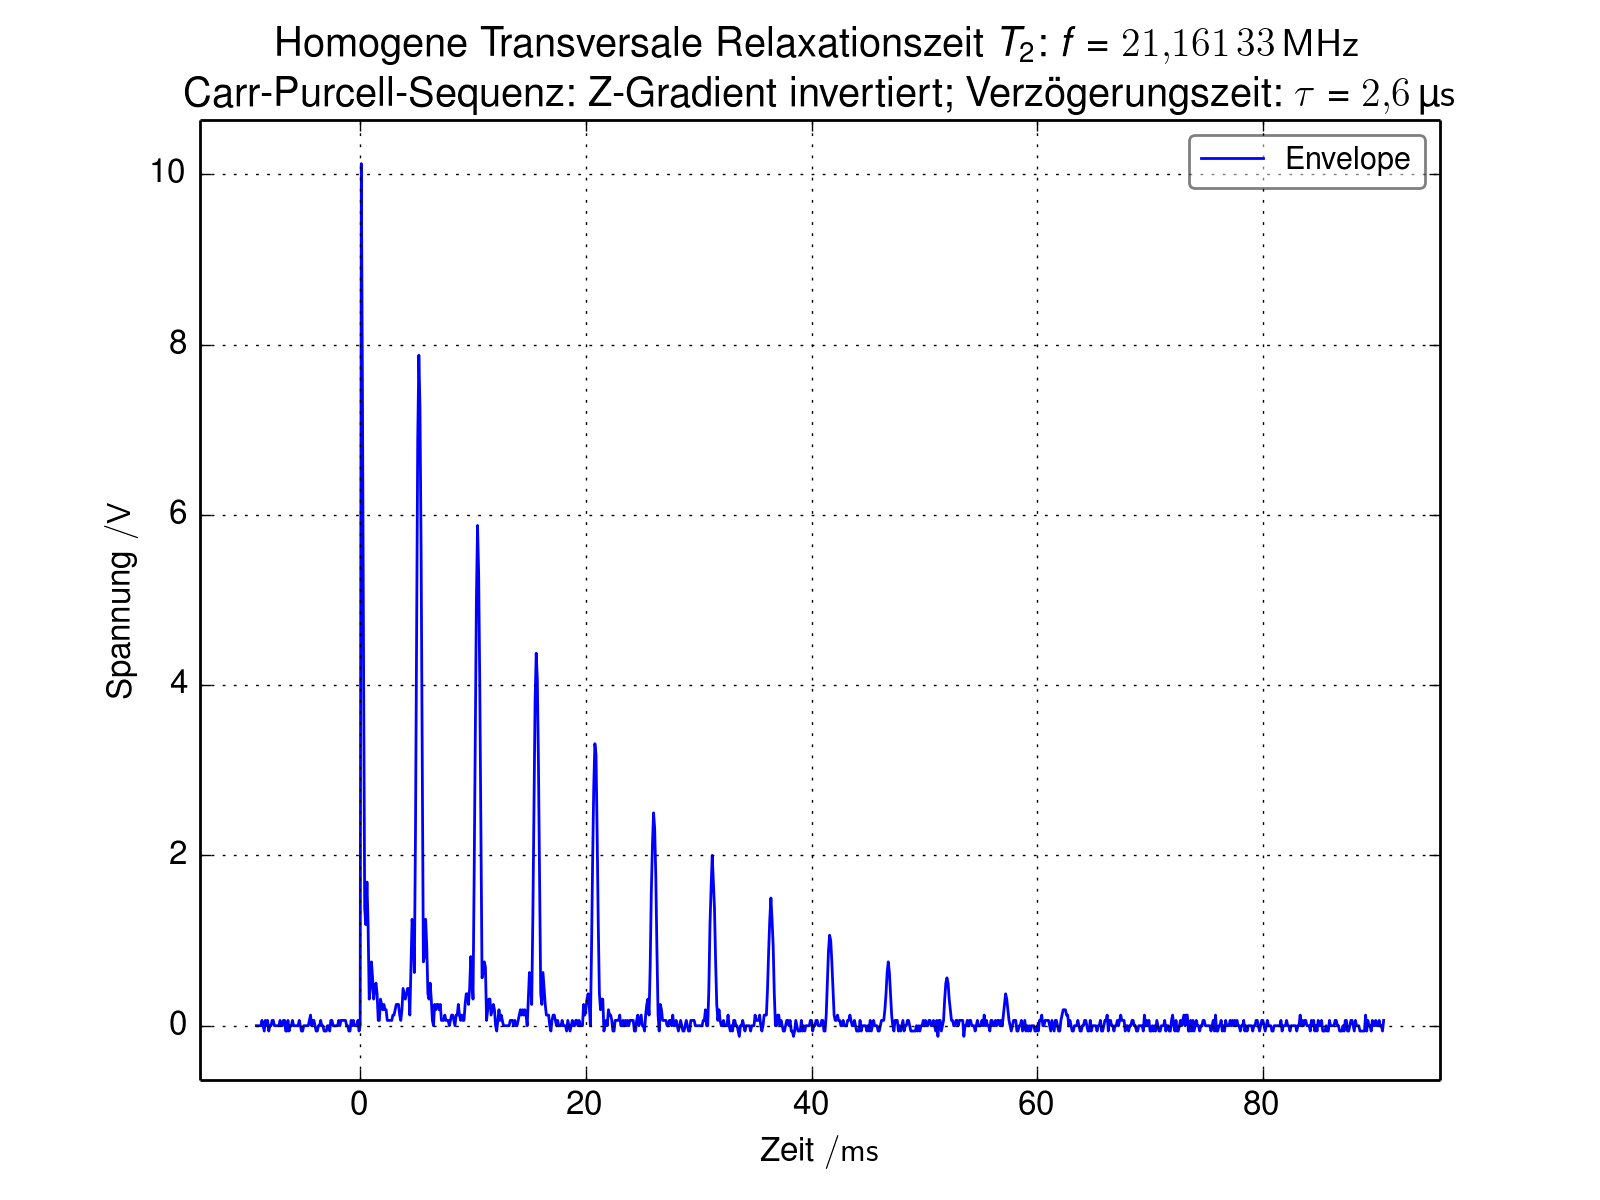
\includegraphics[width=\textwidth]
            {Figures/HomoTransRelax_Carr3.png}
            \caption{bla bla.}
            \label{figCarr3}
          \end{minipage}\quad
          \begin{minipage}{.48\textwidth}
            \centering
            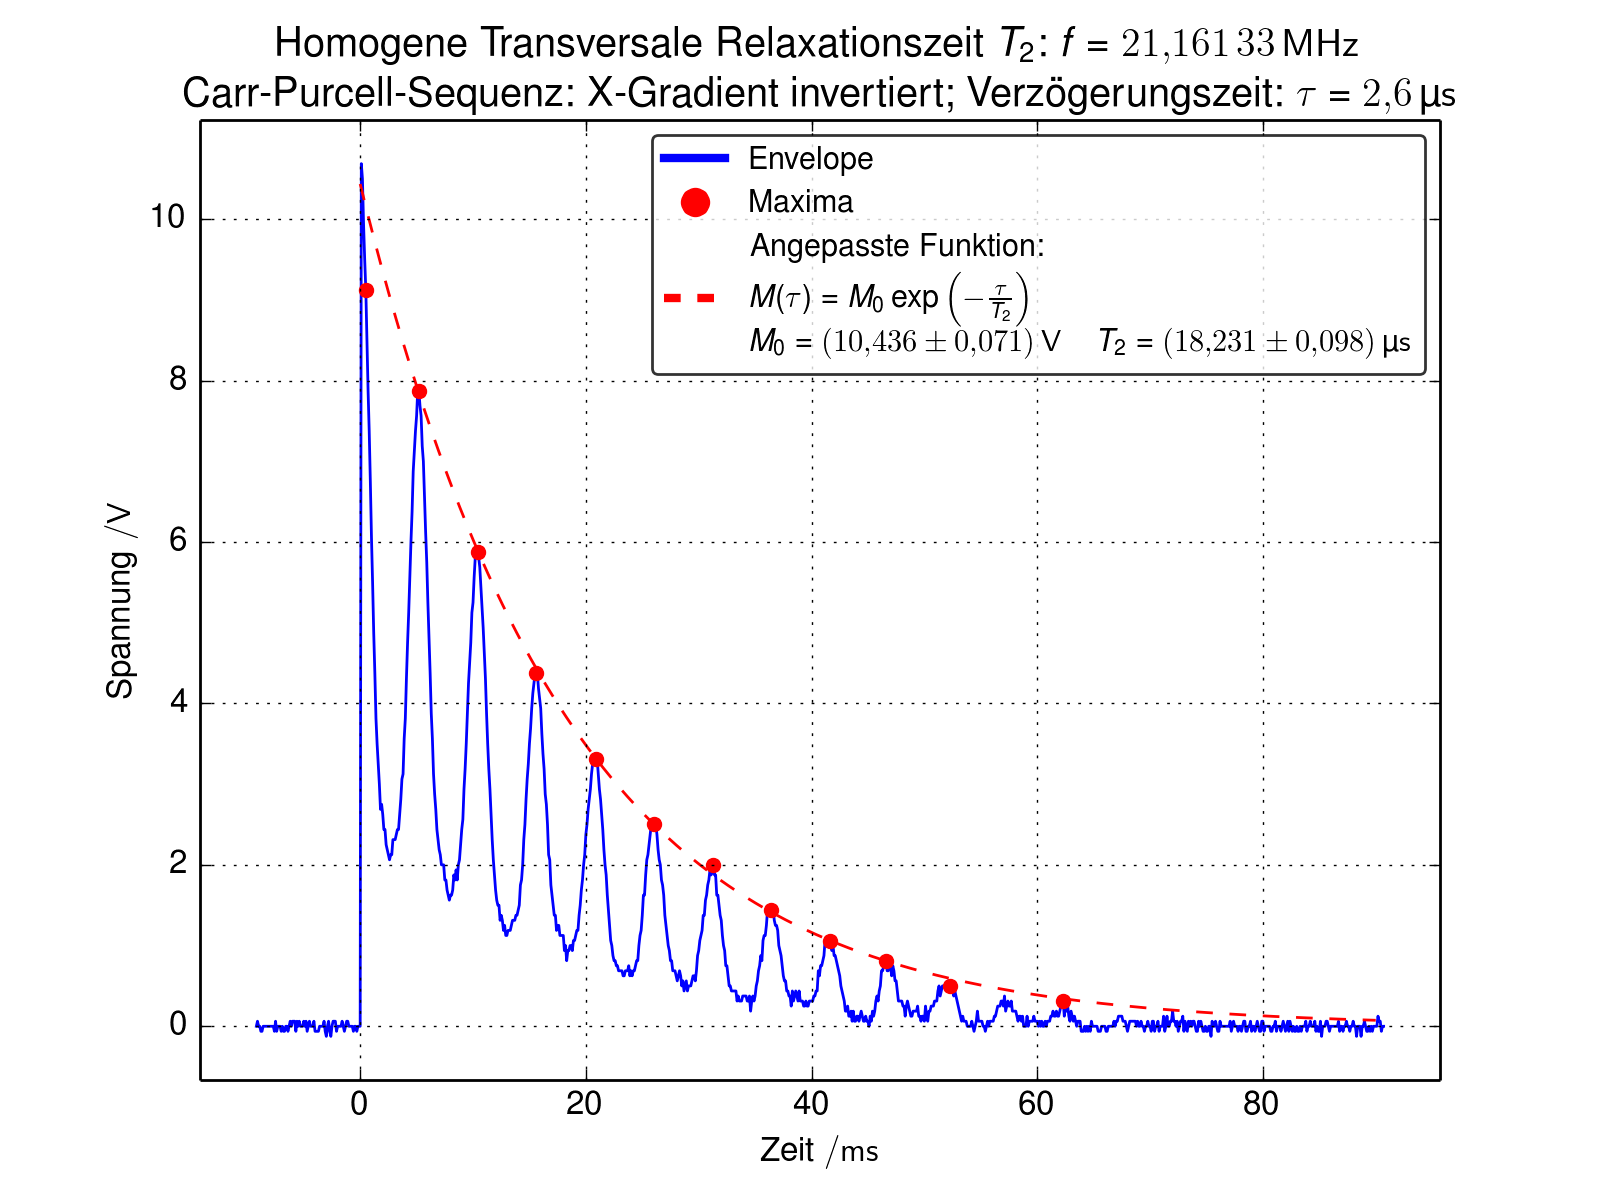
\includegraphics[width=\textwidth]
            {Figures/HomoTransRelax_Carr4.png}
            \caption{bla bla.}
            \label{figCarr4}
          \end{minipage}
        \end{figure}
        
        
      \end{subsection}
      %%%%%%%%%%%%%%%%%%%%%%%%%%%%%%%%%%%%%%%
      
      
      \newpage
      %%%%%%%%%%%%%%%%%%%%%%%%%%%%%%%%%%%%%%%
      %%%%%%%%%%%%%%%%%%%%%%%%%%%%%%%%%%%%%%%
      %%%%%%%%%%%%%%%%%%%%%%%%%%%%%%%%%%%%%%%
      \begin{subsection}{Meiboom-Gill-Spinecho-Sequenz}
        \label{chpHomoTransRelaxMG}
        
        
        
        
        \begin{figure}[htb]
          \centering
          \begin{minipage}{.48\textwidth}
            \centering
            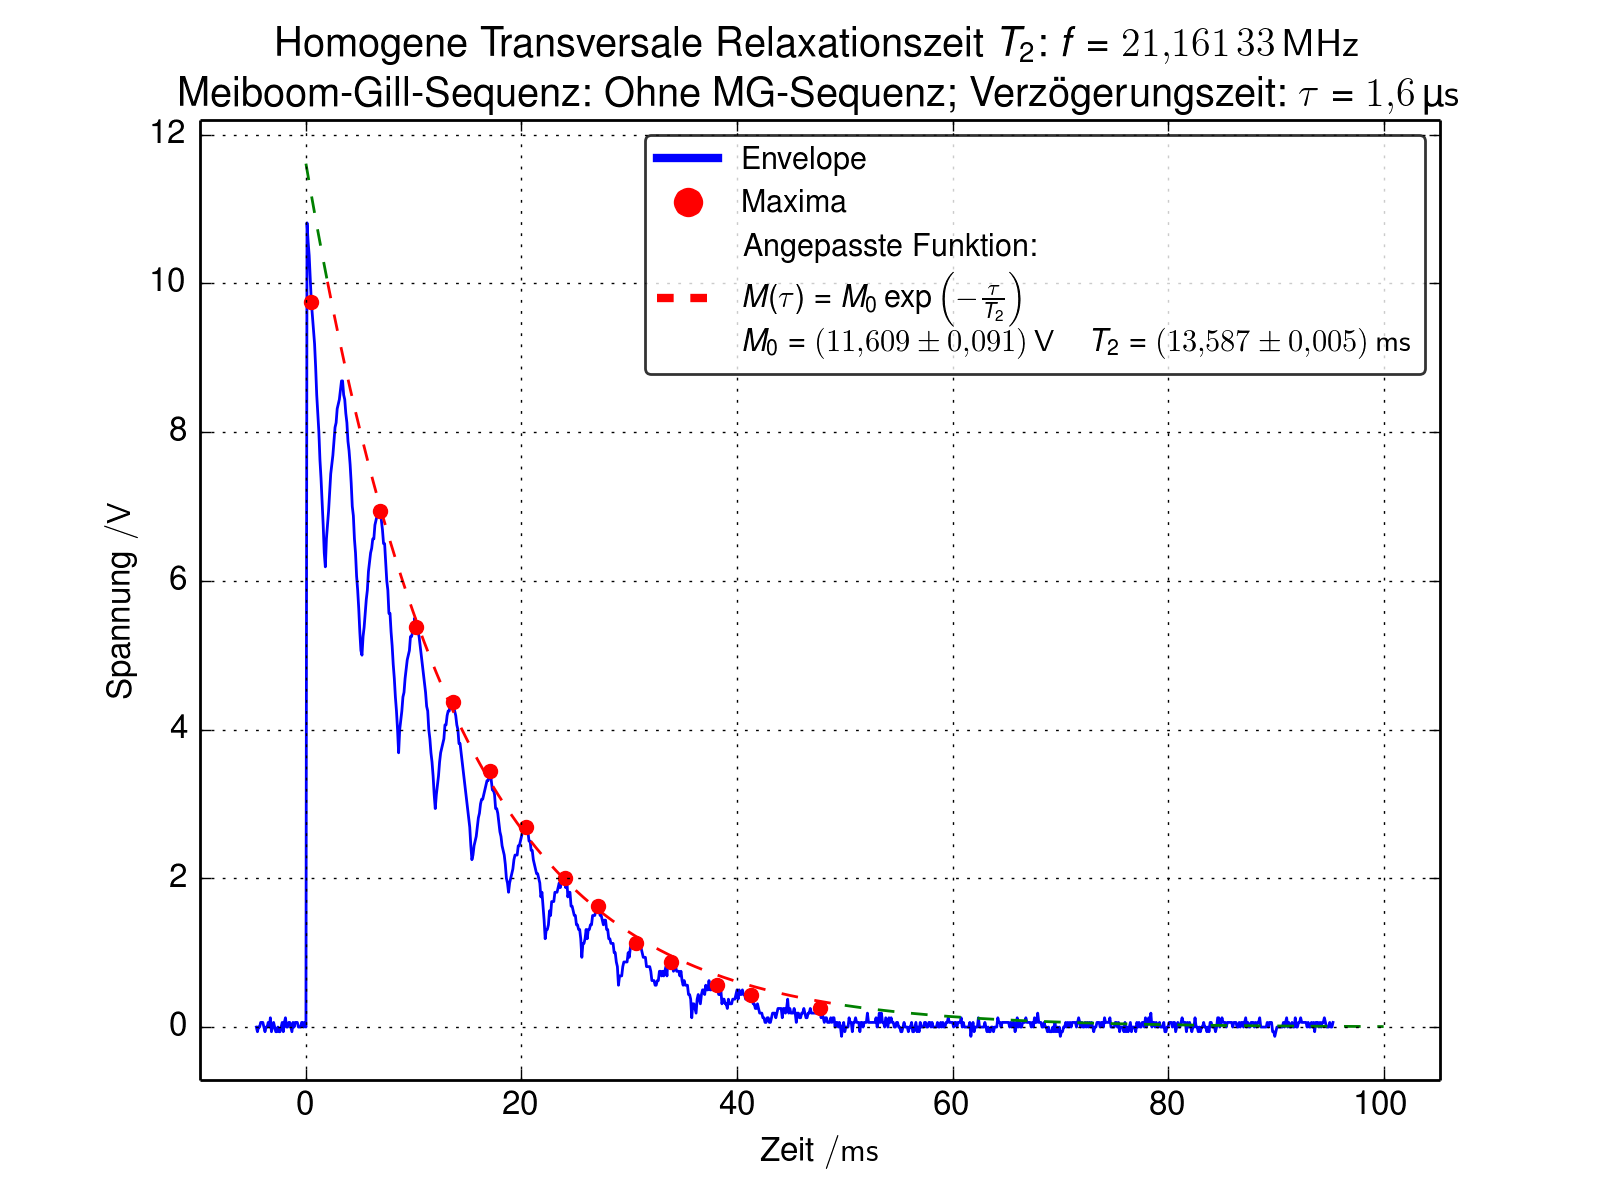
\includegraphics[width=\textwidth]
            {Figures/HomoTransRelax_MG_env0.png}
            \caption{bla bla.}
            \label{figMG_env0}
          \end{minipage}\quad
          \begin{minipage}{.48\textwidth}
            \centering
            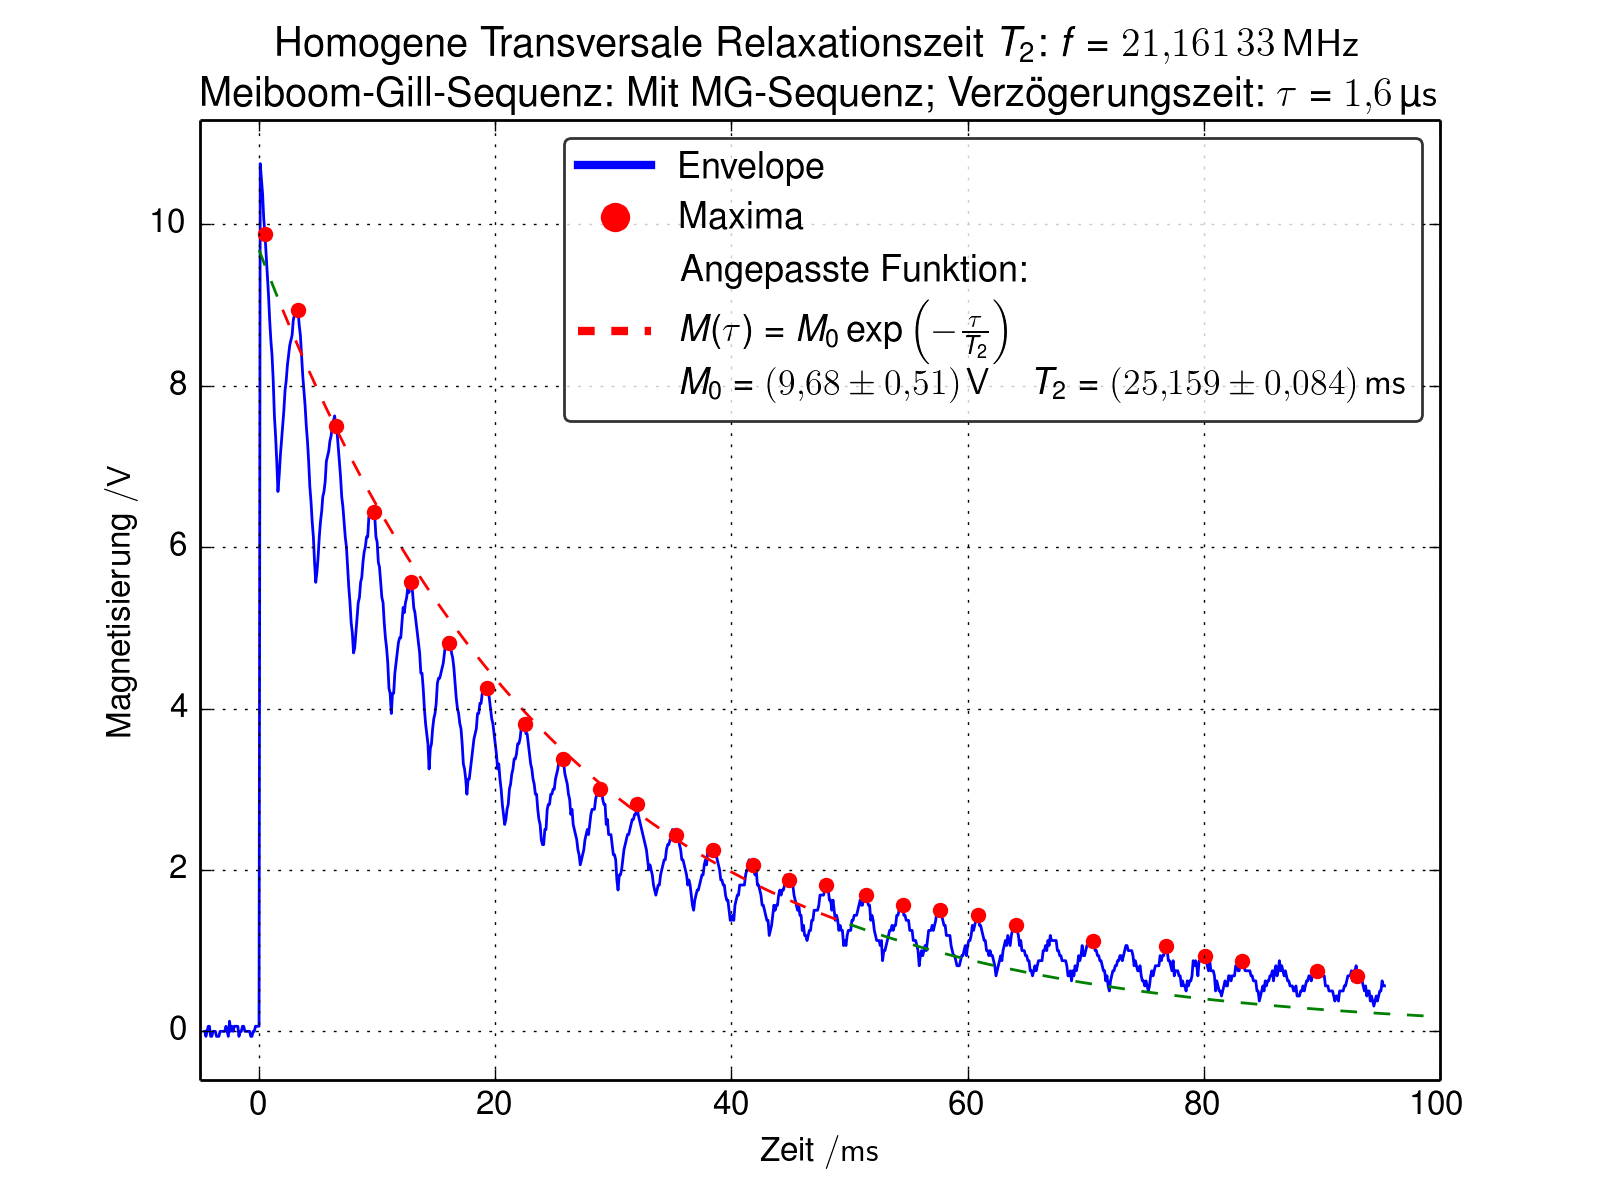
\includegraphics[width=\textwidth]
            {Figures/HomoTransRelax_MG_env1.png}
            \caption{bla bla.}
            \label{figMG_env1}
          \end{minipage}\\
          \begin{minipage}{.48\textwidth}
            \centering
            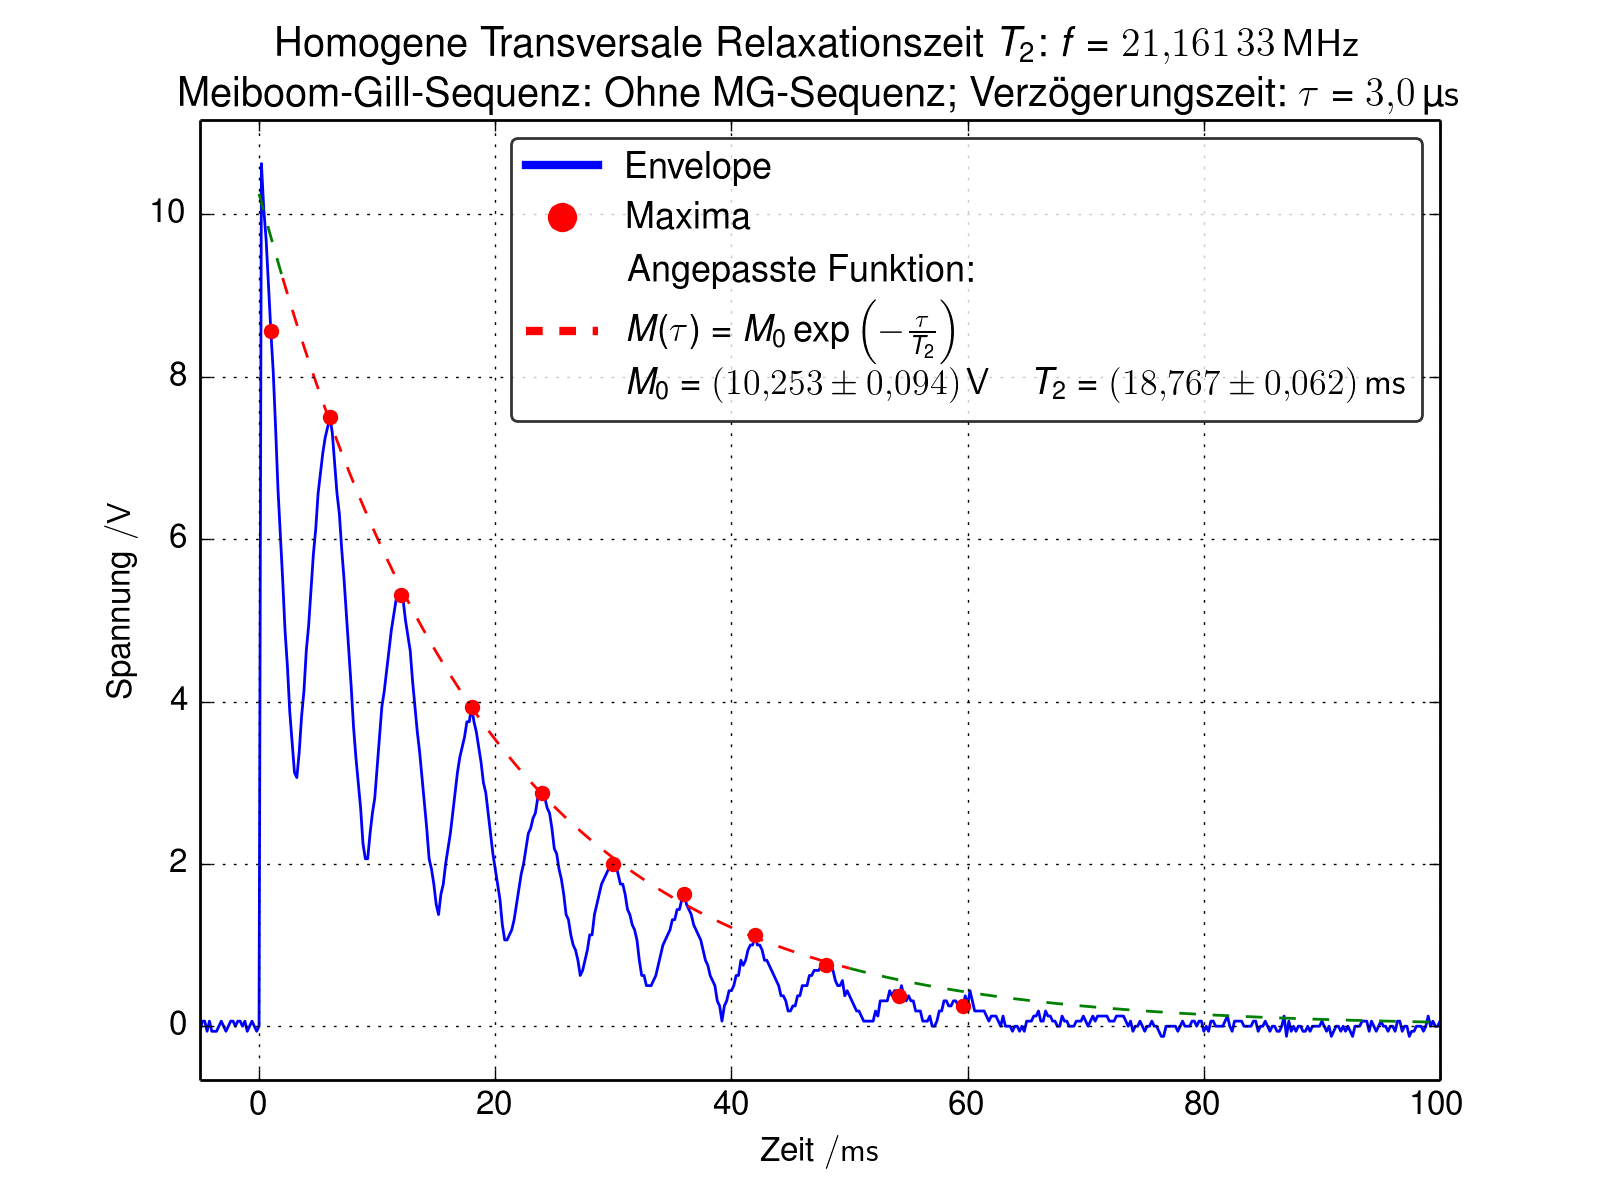
\includegraphics[width=\textwidth]
            {Figures/HomoTransRelax_MG_env2.png}
            \caption{bla bla.}
            \label{figMG_env2}
          \end{minipage}\quad
          \begin{minipage}{.48\textwidth}
            \centering
            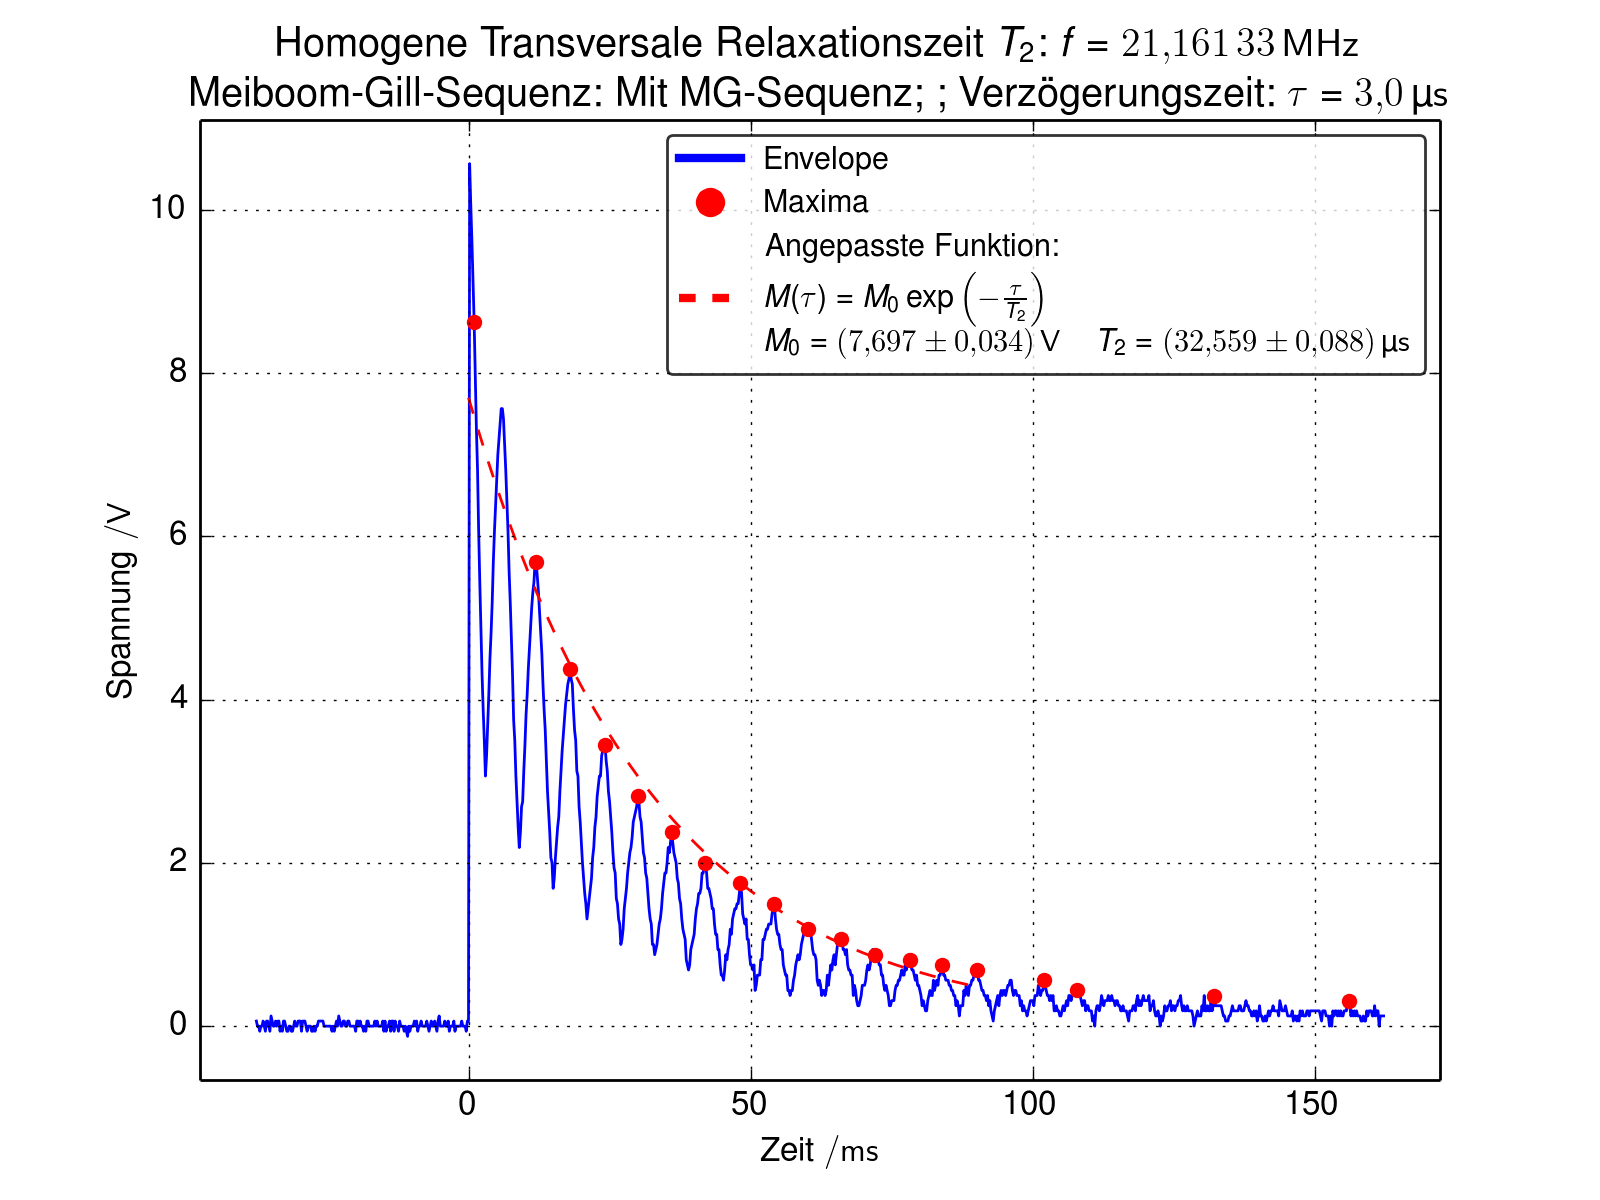
\includegraphics[width=\textwidth]
            {Figures/HomoTransRelax_MG_env3.png}
            \caption{bla bla.}
            \label{figMG_env3}
          \end{minipage}
        \end{figure}
        
        
      \end{subsection}
      %%%%%%%%%%%%%%%%%%%%%%%%%%%%%%%%%%%%%%%
      
    \end{section}
    %%%%%%%%%%%%%%%%%%%%%%%%%%%%%
    
    
    
    \newpage
    %%%%%%%%%%%%%%%%%%%%%%%%%%%%%
    %%%%%%%%%%%%%%%%%%%%%%%%%%%%%
    %%%%%%%%%%%%%%%%%%%%%%%%%%%%%
    \begin{section}{Diskussion}
      \label{chpAuswertungDiskussion}
      
      
      
    \end{section}
    %%%%%%%%%%%%%%%%%%%%%%%%%%%%%
   
  \end{chapter}
  %%%%%%%%%%%%%%%%%%%%
  
  
  
  %%%%%%%%%%%%%%%%%%%%
  %%%%%%%%%%%%%%%%%%%%
  %%%%%%%%%%%%%%%%%%%%
  %%%%%%%%%%%%%%%%%%%%
%%%%%%%%%%%%%%%%%%%%
%%%%%%%%%%%%%%%%%%%%
\begin{appendix}
  \label{Anhang}
  
  
  
  %%%%%%%%%%%%%%%%%%%%%%%%%%%%%%
  %%%%%%%%%%%%%%%%%%%%%%%%%%%%%%
  %%%%%%%%%%%%%%%%%%%%%%%%%%%%%%
  \begin{chapter}{ERSTER TEIL}
    \label{Anhang:chp:ERSTERTEIL}
    
    
    
  \end{chapter}
  %%%%%%%%%%%%%%%%%%%%%%%%%%%%%%
  
  
  
  %%%%%%%%%%%%%%%%%%%%%%%%%%%%%%
  %%%%%%%%%%%%%%%%%%%%%%%%%%%%%%
  %%%%%%%%%%%%%%%%%%%%%%%%%%%%%%
  \begin{chapter}{ZWEITER TEIL}
    \label{Anhang:chp:ZWEITERTEIL}
    
    
    
  \end{chapter}
  %%%%%%%%%%%%%%%%%%%%%%%%%%%%%%
  
\end{appendix}
%%%%%%%%%%%%%%%%%%%%
 
  %%%%%%%%%%%%%%%%%%%%
  
  
  
  %%%%%%%%%%%%%%%%%%%%
  %%%%%%%%%%%%%%%%%%%%
  %%%%%%%%%%%%%%%%%%%%
  \begin{thebibliography}{99}
    \scriptsize
    \bibitem{bib:Anleitung}\url{http://www.praktika.physik.uni-bonn.de/module/physik412/downloads/p441d}
\bibitem{bib:}\url{bla}
  \end{thebibliography}
  %%%%%%%%%%%%%%%%%%%%
 
\end{document}
%%%%%%%%%%
